\documentclass[11pt]{beamer}
\usepackage{xcolor,colortbl}

\usetheme[progressbar=frametitle]{metropolis}
\usepackage{appendixnumberbeamer}
\usepackage[portuguese]{babel}
\usepackage{booktabs}
\usepackage[scale=2]{ccicons}
\usepackage{pgfplots}
\usepgfplotslibrary{dateplot}
\usepackage{hyperref}
\usepackage{subfigure} 
\usepackage{graphicx}
\usepackage{xspace}
\usepackage{natbib}
\newcommand{\themename}{\textbf{\textsc{metropolis}}\xspace}

\usepackage{ragged2e}
\apptocmd{\frame}{}{\justifying}{}

\title{Automata Based Technique for Error-Tolerant Autocompletion}
\subtitle{Edit Vector Automaton Data Structure}
\date{\today}
\author{Anderson Pimentel e Van Den Berg}
\institute{Instituto de Computação (ICOMP) - UFAM}
\titlegraphic{\hfill
\includegraphics[height=1.3cm]{pictures/logo_ufam.png}}

\begin{document}
\maketitle

\begin{frame}{Conteúdo}
  \setbeamertemplate{section in toc}[sections numbered]
  \tableofcontents[hideallsubsections]
\end{frame}

\section{Introdução}

\begin{frame}[fragile]{Arquitetura de Máquina de Busca}

    \begin{figure}
      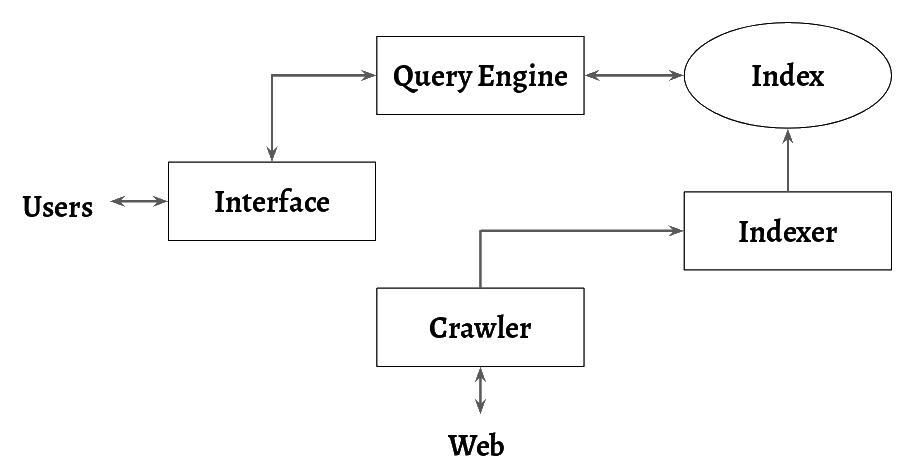
\includegraphics[scale=0.32]{pictures/arquitetura_mb.png}
      \centering
    \end{figure}

\end{frame}

\begin{frame}[fragile]{Arquitetura de Máquina de Busca}

    \begin{figure}
      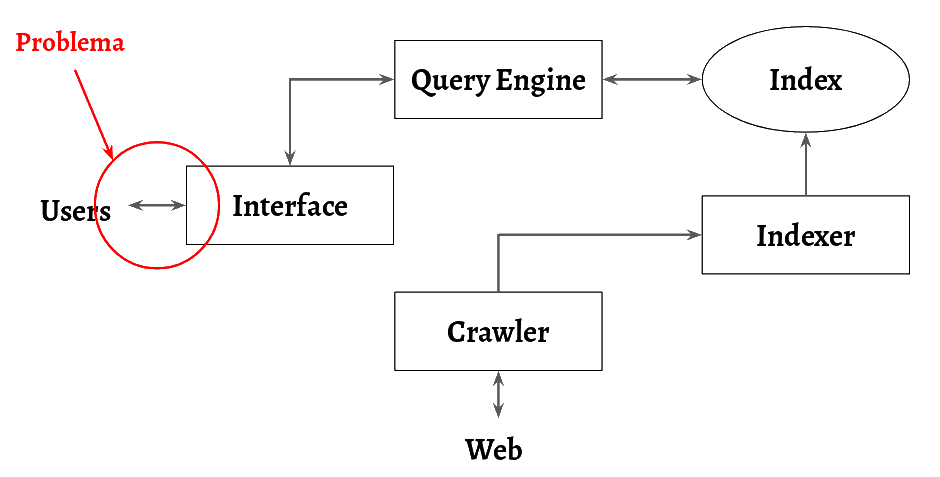
\includegraphics[scale=0.32]{pictures/problema_arquitetura_mb_.png}
      \centering
    \end{figure}
 
\end{frame}

\begin{frame}[fragile]{Exemplos de Problemas}

    \begin{itemize}
        \item Erros de digitação
        \item Erros ortográficos
        \item Pouco conhecimento da base de dados
        \item Abordagem ``tentar e ver''
        \item Resultados ruins
    \end{itemize}
    \pause
    Para resolver estes problemas é utilizado \textbf{algoritmos de autocompletação}. No entanto, algoritmos de autocompletação de consultas ainda têm problemas!
    
\end{frame}

\begin{frame}[fragile]{Exemplos de Problemas em AA}
    
    \begin{itemize}
        \item Erros de digitação
        \item Erros ortográficos
        \item Atrasos de internet
    \end{itemize}
    
    Algoritmos de autocompletação tradicionais não permitem erros de entrada.
    
    \pause
    Para resolver estes problemas é utilizado técnicas de \textbf{tolerância a erros} capazes de responder \textbf{rapidamente} em poucos ms.

\end{frame}

\begin{frame}{Velocidade de Resposta}
    \begin{itemize}
        \justifying
        \item Cada consulta necessita obter sugestões em menos de 100ms [Ji et al. 2009] para evitar atrasos perceptíveis durante a sessão interativa de busca. \pause
        \item O tempo de resposta pode ser influenciado por outros fatores, tais como: congestionamento na rede, renderização do JS. \pause
        \item Diante disto, os algoritmos de autocompletação devem ser cada vez mais rápidos e ainda assim tratar possíveis erros de entrada.
    \end{itemize}

\end{frame}

\section{Árvores digitais}

\begin{frame}[fragile]{Árvores Digitais}

    \textbf{Definição:} É uma estrutura de dados do tipo árvore ordenada, que pode ser usada para armazenar um array associativo em que as chaves são normalmente cadeias de caracteres. (Wikipédia - https://pt.wikipedia.org/wiki/Trie)

    \pause
    \begin{figure}
      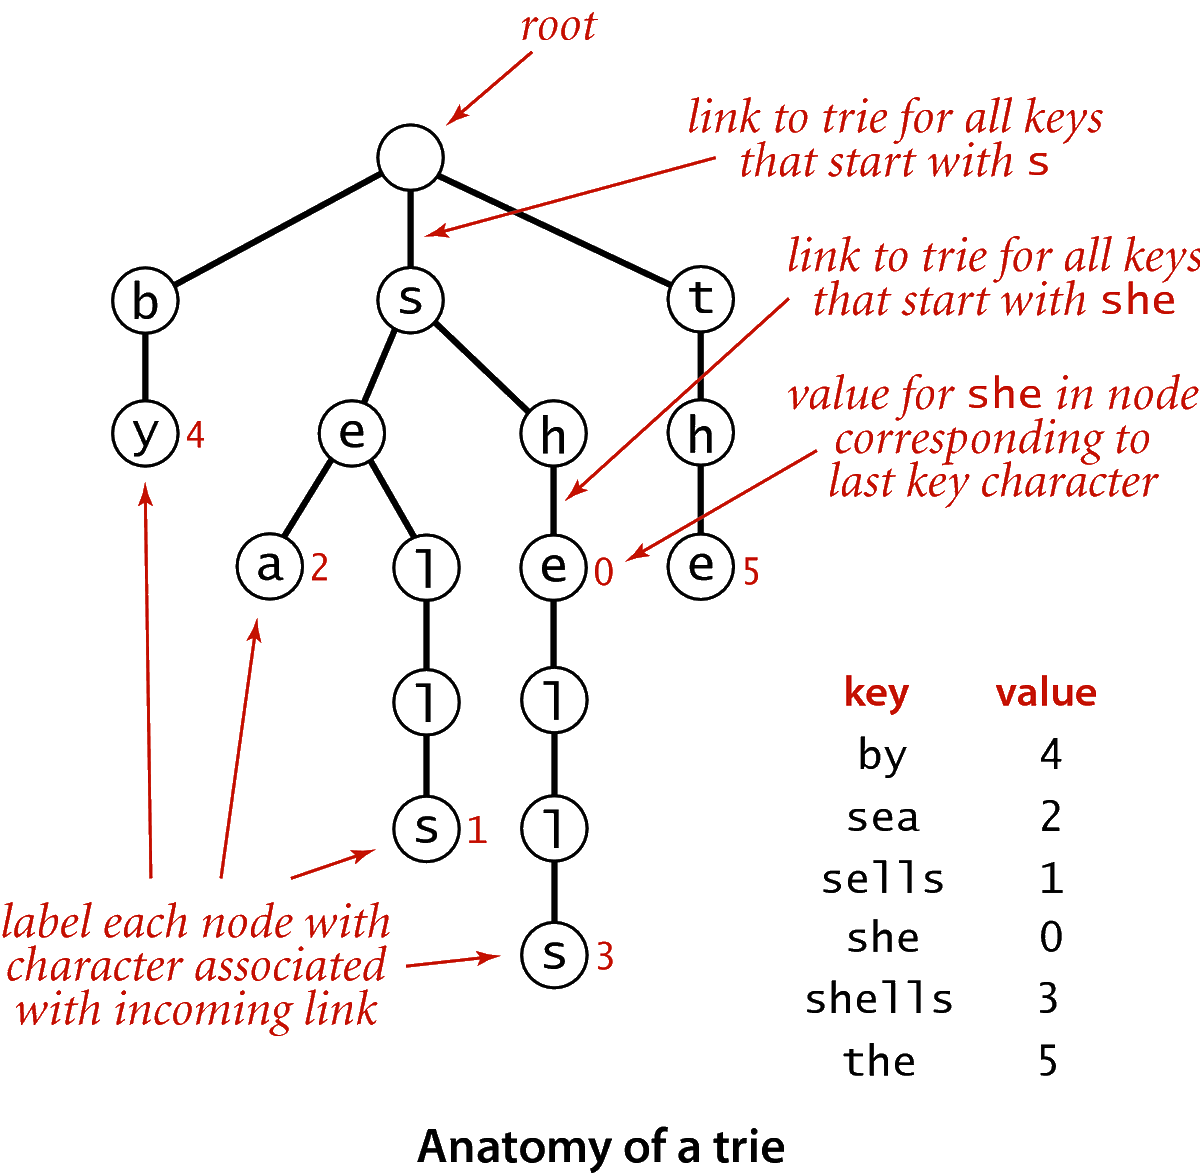
\includegraphics[scale=0.13]{pictures/trie_anatomy.png}
      \centering
    \end{figure}

\end{frame}

\begin{frame}[fragile]{Árvores Digitais}

    Demonstração: \href{https://www.cs.usfca.edu/~galles/visualization/Trie.html}{\color{blue}\underline{Inicialização dos nós}}

\end{frame}

\section{Tolerância a erros}

\begin{frame}{Tolerância a erros}
	\begin{itemize}
	    \justifying
		\item Permite uma pequena quantidade de erros (usualmente controlado por um limiar $\tau$ chamado distância de edição). \pause
		\item Exemplo: Se um usuário digita um prefixo incorreto \textbf{Schwarzenegger} tal como \textbf{Shwarz}, \textbf{Schwarzenegger} será sugerido se é permitido uma edição de erro no prefixo correspondente [Chaudhuri and Kaushik 2009]. 
	\end{itemize}
\end{frame}

\begin{frame}{Tolerância a erros}
	\begin{itemize}
		\item A função \textbf{ed(s, t)} retorna as distâncias de edição entre duas strings \textbf{s} e \textbf{t}, no qual mede o número mínimo de operações de edição, incluindo inserção, exclusão e substituição de um caractere, para transformar \textbf{s} em \textbf{t}. \pause
		\item \textbf{Definição:} Dado uma coleção de palavras $S$, uma consulta $q$, e um limiar de distância de edição $\tau$, a autocompletação de consulta com tolerância a erro deve retornar todas as palavras $s \in S$, tal que $\exists s' \leq s$ onde $s'=s[1 \ldots |s'|], ed(s', q) \leq \tau$. Os resultados são computados incrementalmente conforme o usuário modifica a consulta.
	\end{itemize}
\end{frame}

\begin{frame}{Tolerância a erros}
	\begin{itemize}
		\item S = [bola, bolo, bala]. 
		\item s’ = [ [b, bo, bol, bola], [b, bo, bol, bolo], [b, ba, bal, bala] ]
		\item q = ``bolq''.
		\item $\tau = 1$.
	\end{itemize}
	
	\pause
	\textbf{ed(b, bolq) = ? | ed(bo, bolq) = ? | ed(bol, bolq) = ? | ed(bola, bolq) = ?}
	
    \textbf{ed(b, bolq) = ? | ed(bo, bolq) = ? | ed(bol, bolq) = ? | ed(bolo, bolq) = ?}
    
    \textbf{ed(b, bolq) = ? | ed(ba, bolq) = ? | ed(bal, bolq) = ? | ed(bala, bolq) = ?}
\end{frame}

\begin{frame}{Tolerância a erros}
	\begin{itemize}
		\item S = [bola, bolo, bala]. 
		\item s’ = [ [b, bo, bol, bola], [b, bo, bol, bolo], [b, ba, bal, bala] ]
		\item q = ``bolq''.
		\item $\tau = 1$.
	\end{itemize}
	
	\textbf{ed(b, bolq) = 3 | ed(bo, bolq) = 2 | ed(bol, bolq) = 1 | ed(bola, bolq) = 1}
	
    \textbf{ed(b, bolq) = ? | ed(bo, bolq) = ? | ed(bol, bolq) = ? | ed(bolo, bolq) = ?}
    
    \textbf{ed(b, bolq) = ? | ed(ba, bolq) = ? | ed(bal, bolq) = ? | ed(bala, bolq) = ?}
\end{frame}

\begin{frame}{Tolerância a erros}
	\begin{itemize}
		\item S = [bola, bolo, bala]. 
		\item s’ = [ [b, bo, bol, bola], [b, bo, bol, bolo], [b, ba, bal, bala] ]
		\item q = ``bolq''.
		\item $\tau = 1$.
	\end{itemize}
	
	\textbf{ed(b, bolq) = 3 | ed(bo, bolq) = 2 | ed(bol, bolq) = 1 | ed(bola, bolq) = 1}
	
    \textbf{ed(b, bolq) = 3 | ed(bo, bolq) = 2 | ed(bol, bolq) = 1 | ed(bolo, bolq) = 1}
    
    \textbf{ed(b, bolq) = ? | ed(ba, bolq) = ? | ed(bal, bolq) = ? | ed(bala, bolq) = ?}
\end{frame}

\begin{frame}{Tolerância a erros}
	\begin{itemize}
		\item S = [bola, bolo, bala]. 
		\item s’ = [ [b, bo, bol, bola], [b, bo, bol, bolo], [b, ba, bal, bala] ]
		\item q = ``bolq''.
		\item $\tau = 1$.
	\end{itemize}
	
	\textbf{ed(b, bolq) = 3 | ed(bo, bolq) = 2 | ed(bol, bolq) = 1 | ed(bola, bolq) = 1}
	
    \textbf{ed(b, bolq) = 3 | ed(bo, bolq) = 2 | ed(bol, bolq) = 1 | ed(bolo, bolq) = 1}
    
    \textbf{ed(b, bolq) = 3 | ed(ba, bolq) = 3 | ed(bal, bolq) = 2 | ed(bala, bolq) = 2}
    
    \pause
    \begin{itemize}
        \item Resposta = [bola, bolo]
    \end{itemize}
\end{frame}

\begin{frame}{Tolerância a erros}
    \begin{figure}
        \centering
        \subfigure[Busca por shwarzenegger]{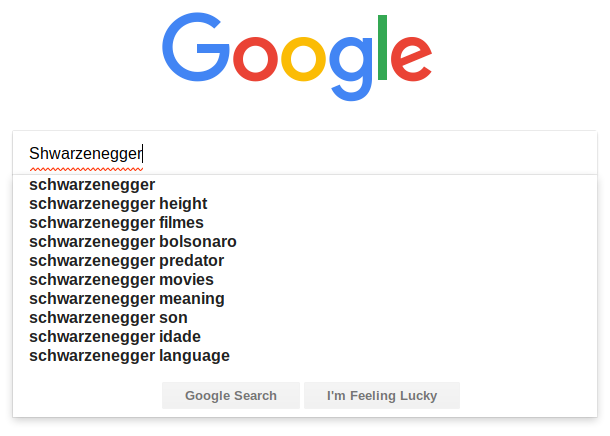
\includegraphics[width=0.45\textwidth]{pictures/schwarzenegger.png}}
        \subfigure[Busca por bolq]{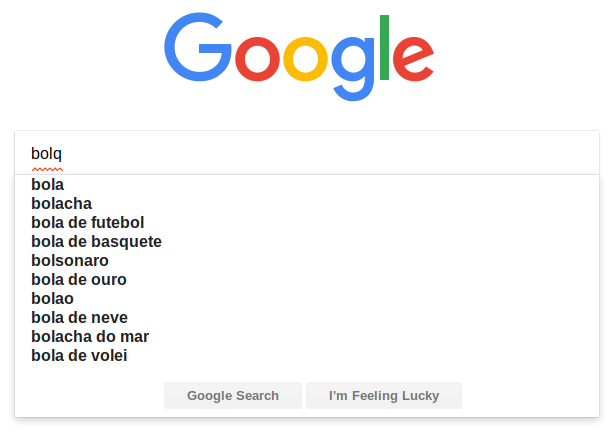
\includegraphics[width=0.45\textwidth]{pictures/bolq.png}}
        \caption{Tolerância a erro no Google}
        \label{fig:fig}
    \end{figure}

\end{frame}

\section{Principais algoritmos}

\begin{frame}{Principais algoritmos}
    
   \begin{itemize}
		\item \textbf{$\big[ \text{ICAN} \big]$ S. Ji, G. Li, C.Li, and J. Feng. Efficient interactive fuzzy keyword search, 2009}
		\item \textbf{$\big[ \text{ICPAN} \big]$ S. Ji, G. Li, C.Li, and J. Feng. Efficient fuzzy full-text type-ahead search, 2011.}
		\item $\big[ \text{IncNGTrie} \big]$ C. Xiao, J. Qin, W. Wang, Y. Ishikawa, K. Tsuda, and K. Sadakane. Efficient error-tolerant query autocompletion, 2013.
		\item $\big[ \text{PIVOTAL} \big]$ D. Deng, G. Li, and J. Feng. A pivotal prefix based filtering algorithm for string similarity search, 2014.
    \end{itemize} 
    
\end{frame}

\begin{frame}{Principais algoritmos}
    
   \begin{itemize}
		\item $\big[ \text{HSTRee} \big]$ J. Wang, G. Li, D. Deng, Y. Zhang, and J. Feng. Two birds with one stone: An efficient hierarchical framework for top-k and threshold-based string similarity search, 2015.
		\item $\big[ \text{META} \big]$ D. Deng, G. Li, H. Wen, H. V. Jagadish, and J. Feng. META: An Efficient Matching-Based Method for Error-Tolerant Autocompletion, 2016.
        \item \textbf{$\big[ \text{BEVA} \big]$ C. Xiao, J. Qin, and W. Wang. BEVA: An efficient Query Processing algorithm for Error-Tolerant Autocompletion, 2016.}
    \end{itemize} 
    
\end{frame}

\subsection{ICAN}

\begin{frame}{[ICAN] Efficient interactive fuzzy keyword search, \cite{ICAN}.}

    Possui duas funcionalidades: 

    \begin{enumerate}
        \item \textbf{Interactive:} O sistema busca pelas melhores respostas em tempo real (on the fly) na medida que o usuário digita palavras da consulta. \pause
        \item \textbf{Fuzzy:} Quando é buscado por registros relevantes, o sistema tenta também buscar registros que incluem palavras similares para as palavras da consulta, até mesmo se não são exatamente iguais. \pause
    \end{enumerate}
    
    São abordados técnicas para \textbf{prefixo único} e \textbf{prefixo com múltiplas palavras}.
    
\end{frame}

\begin{frame}{[ICAN] Efficient interactive fuzzy keyword search, 2009}

    \small
    Suponhamos que $\tau = 2$. Um usuário digita um prefixo \textit{p} = ``nlis''. Os prefixos ``li'', ``lin'', ``liu'' e ``luis'' são todos similares para \textit{p}. \pause

    \begin{figure}
      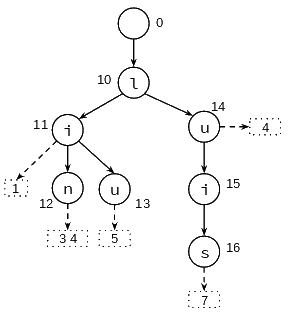
\includegraphics[scale=0.50]{pictures/ican_1.png}
      \centering
    \end{figure}
    
\end{frame}

\begin{frame}{[ICAN] Efficient interactive fuzzy keyword search, 2009}
    
    \small
    Suponhamos que $\tau = 2$. Um usuário digita um prefixo \textit{p} = ``nlis''. Os prefixos ``li'', ``lin'', ``liu'' e ``luis'' são todos similares para \textit{p}.

    \begin{figure}
      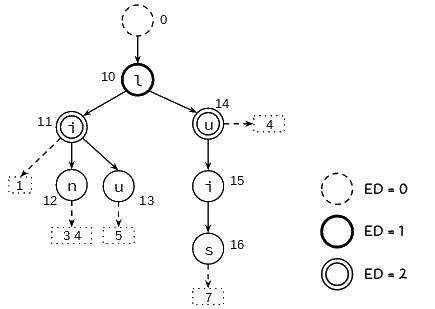
\includegraphics[scale=0.45]{pictures/ican_2.png}
      \centering
    \end{figure}
    
    \textbf{1) Inicialização}
    
\end{frame}


\begin{frame}{[ICAN] Efficient interactive fuzzy keyword search, 2009.}

    \small
    Suponhamos que $\tau = 2$. Um usuário digita um prefixo \textit{p} = ``nlis''. Os prefixos ``li'', ``lin'', ``liu'' e ``luis'' são todos similares para \textit{p}.
    
    \begin{figure}
      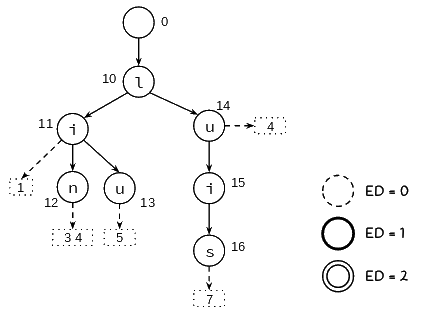
\includegraphics[scale=0.45]{pictures/ican_default.png}
      \centering
    \end{figure}
    
    \textbf{2) query ``n''}
    
\end{frame}

\begin{frame}{[ICAN] Efficient interactive fuzzy keyword search, 2009.}

    \small
    Suponhamos que $\tau = 2$. Um usuário digita um prefixo \textit{p} = ``nlis''. Os prefixos ``li'', ``lin'', ``liu'' e ``luis'' são todos similares para \textit{p}.
    
    \begin{figure}
      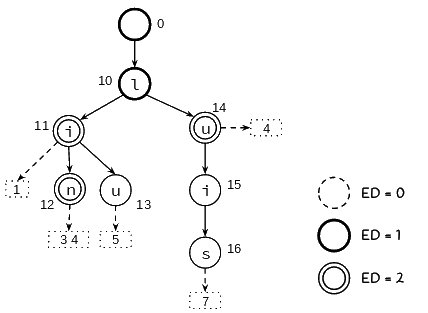
\includegraphics[scale=0.45]{pictures/ican_3.png}
      \centering
    \end{figure}
    
    \textbf{2) query ``n''}
    
\end{frame}

\begin{frame}{[ICAN] Efficient interactive fuzzy keyword search, 2009}

    \small
    Suponhamos que $\tau = 2$. Um usuário digita um prefixo \textit{p} = ``nlis''. Os prefixos ``li'', ``lin'', ``liu'' e ``luis'' são todos similares para \textit{p}.
    
    \begin{figure}
      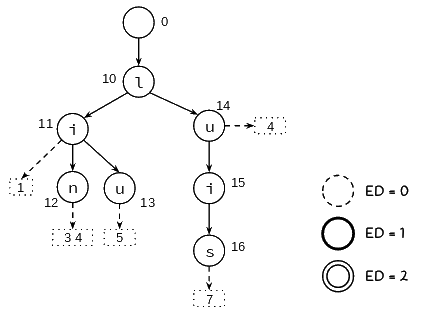
\includegraphics[scale=0.45]{pictures/ican_default.png}
      \centering
    \end{figure}
    
    \textbf{3) query ``nl''}
    
\end{frame}

\begin{frame}{[ICAN] Efficient interactive fuzzy keyword search, 2009}

    \small
    Suponhamos que $\tau = 2$. Um usuário digita um prefixo \textit{p} = ``nlis''. Os prefixos ``li'', ``lin'', ``liu'' e ``luis'' são todos similares para \textit{p}.
    
    \begin{figure}
      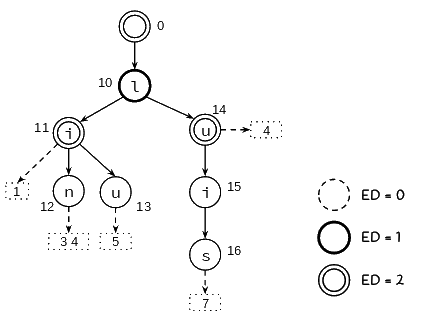
\includegraphics[scale=0.45]{pictures/ican_4.png}
      \centering
    \end{figure}
    
    \textbf{3) query ``nl''}
    
\end{frame}

\begin{frame}{[ICAN] Efficient interactive fuzzy keyword search, 2009}

    \small
    Suponhamos que $\tau = 2$. Um usuário digita um prefixo \textit{p} = ``nlis''. Os prefixos ``li'', ``lin'', ``liu'' e ``luis'' são todos similares para \textit{p}.
    
    \begin{figure}
      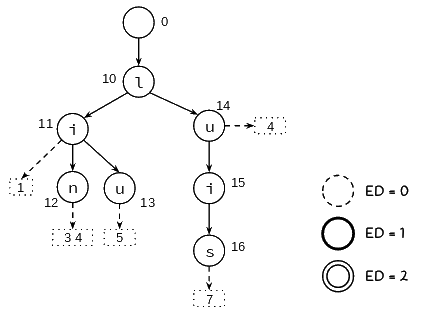
\includegraphics[scale=0.45]{pictures/ican_default.png}
      \centering
    \end{figure}
    
    \textbf{4) query ``nli''}
    
\end{frame}

\begin{frame}{[ICAN] Efficient interactive fuzzy keyword search, 2009}

    \small
    Suponhamos que $\tau = 2$. Um usuário digita um prefixo \textit{p} = ``nlis''. Os prefixos ``li'', ``lin'', ``liu'' e ``luis'' são todos similares para \textit{p}.
    
    \begin{figure}
      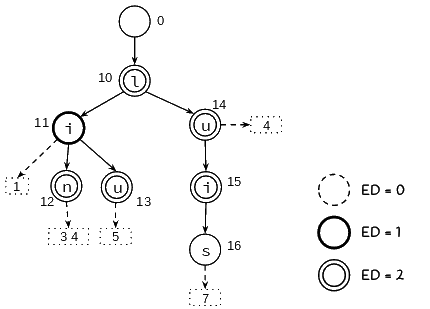
\includegraphics[scale=0.45]{pictures/ican_5.png}
      \centering
    \end{figure}
    
    \textbf{4) query ``nli''}
    
\end{frame}

\begin{frame}{[ICAN] Efficient interactive fuzzy keyword search, 2009}

    \small
    Suponhamos que $\tau = 2$. Um usuário digita um prefixo \textit{p} = ``nlis''. Os prefixos ``li'', ``lin'', ``liu'' e ``luis'' são todos similares para \textit{p}.
    
    \begin{figure}
      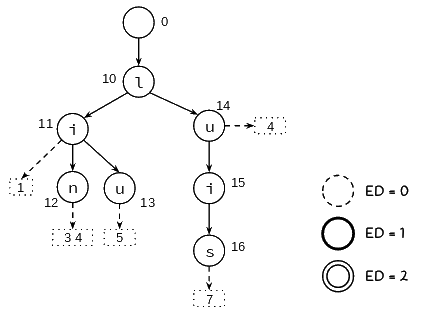
\includegraphics[scale=0.45]{pictures/ican_default.png}
      \centering
    \end{figure}
    
    \textbf{5) query ``nlis''}
    
\end{frame}

\begin{frame}{[ICAN] Efficient interactive fuzzy keyword search, 2009}

    \small
    Suponhamos que $\tau = 2$. Um usuário digita um prefixo \textit{p} = ``nlis''. Os prefixos ``li'', ``lin'', ``liu'' e ``luis'' são todos similares para \textit{p}.
    
    \begin{figure}
      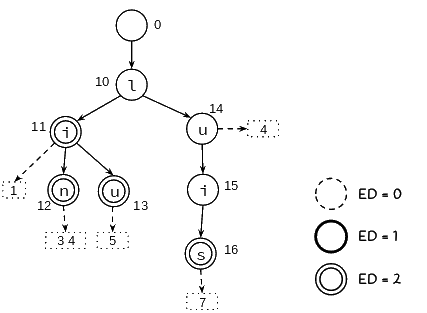
\includegraphics[scale=0.45]{pictures/ican_6.png}
      \centering
    \end{figure}
    
    \textbf{5) query ``nlis''}
    
\end{frame}

\begin{frame}{[ICAN] Efficient interactive fuzzy keyword search, 2009}

    \small
    Suponhamos que $\tau = 2$. Um usuário digita um prefixo \textit{p} = ``nlis''. Os prefixos ``li'', ``lin'', ``liu'' e ``luis'' são todos similares para \textit{p}.
    
    \begin{figure}
      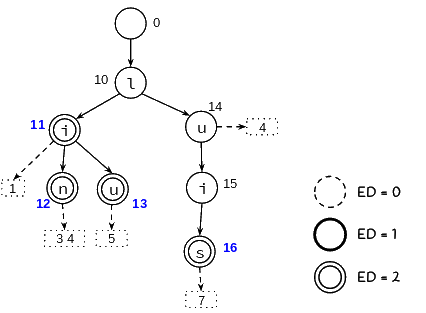
\includegraphics[scale=0.45]{pictures/ican_7.png}
      \centering
    \end{figure}
    
    Assim, os nós 11, 12, 13 e 16 são \textbf{nós ativos} para \textit{p}.
    
\end{frame}

\begin{frame}{[ICAN] Efficient interactive fuzzy keyword search, 2009}

    Para realizar a computação incremental dos nós ativos (ICAN) quando o usuário digita letra por letra foi desenvolvido um algoritmo baseado em \textit{caching}. \pause
    
    Dado um prefixo de entrada \textit{p}, é computado e guardado o conjunto dos nós ativos $\Phi_p = \big\{ \big \langle n, \xi_n \big \rangle \big\}$, no qual $n$ é um nó ativo, e $\xi_n = ed \big(p, n \big) \le \tau$.  \pause
    
    Assim, quando o usuário digita uma letra a mais depois de \textit{p}, os nós ativos de \textit{p} podem ser usados para computar os nós ativos da nova consulta.
    
\end{frame}

\begin{frame}{[ICAN] Efficient interactive fuzzy keyword search, 2009}

    Passos:
    
    \begin{enumerate}
        \item Para cada $\big\langle n, \xi_{n} \big\rangle$ em $\Phi_{p_x}$, os descendentes de $n$ são examinados como candidatos a nós ativos para $p_{x+1}$.
        \item Para o nó $n$, se $\xi_{n+1} \le \tau$, então $n$ é um nó ativo  para $p_{x+1}$, e $\big\langle n, \xi_{n+1} \big\rangle$ é adicionado para $\Phi_{p_{x+1}}$
    \end{enumerate}
\end{frame}

\begin{frame}{[ICAN] Efficient interactive fuzzy keyword search, 2009}

    \small
    Suponhamos que $\tau = 2$. Um usuário digita um prefixo \textit{p} = ``nlis''. Os prefixos ``li'', ``lin'', ``liu'' e ``luis'' são todos similares para \textit{p}. \pause

    \begin{figure}
      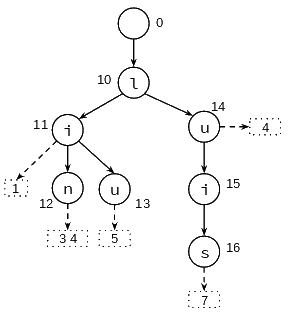
\includegraphics[scale=0.50]{pictures/ican_1.png}
      \centering
    \end{figure}
    
\end{frame}

\begin{frame}{[ICAN] Efficient interactive fuzzy keyword search, 2009}
    
    \begin{figure}
      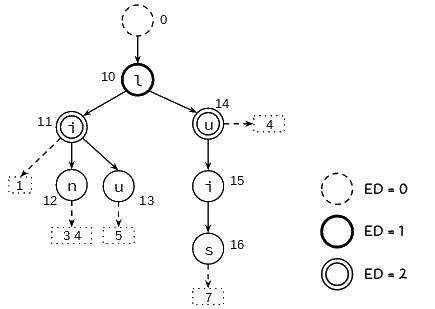
\includegraphics[scale=0.45]{pictures/ican_2.png}
      \centering
    \end{figure}
    
    \textbf{1) Inicialização}
    
\end{frame}

\begin{frame}{[ICAN] Efficient interactive fuzzy keyword search, 2009.}

    \begin{figure}
      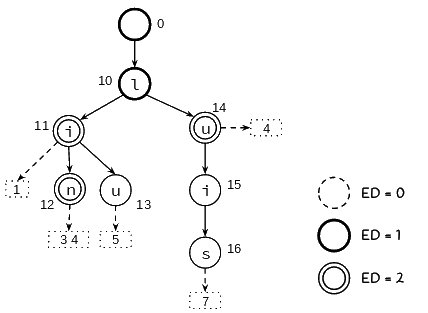
\includegraphics[scale=0.45]{pictures/ican_3.png}
      \centering
    \end{figure}
    
    \textbf{2) query ``n''}
    
    $\Phi_{p_{x}} = \big\{ \big \langle 0, 0 \big \rangle, \big \langle 10, 1 \big \rangle, \big \langle 11, 2 \big \rangle, \big \langle 14, 2 \big \rangle \big\}$
    
    $\Phi_{p_{x+1}} = \big\{ \big \langle 0, 1 \big \rangle, \big \langle 10, 1 \big \rangle, \big \langle 11, 2 \big \rangle, \big \langle 12, 2 \big \rangle, \big \langle 14, 2 \big \rangle \big\}$
    
\end{frame}

\begin{frame}{[ICAN] Efficient interactive fuzzy keyword search, 2009}

    \begin{figure}
      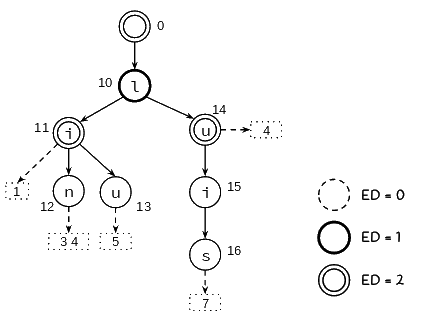
\includegraphics[scale=0.45]{pictures/ican_4.png}
      \centering
    \end{figure}
    
    \textbf{3) query ``nl''}
    
    $\Phi_{p_{x}} = \big\{ \big \langle 0, 1 \big \rangle, \big \langle 10, 1 \big \rangle, \big \langle 11, 2 \big \rangle, \big \langle 12, 2 \big \rangle, \big \langle 14, 2 \big \rangle \big\}$
    
    $\Phi_{p_{x+1}} = \big\{ \big \langle 0, 2 \big \rangle, \big \langle 10, 1 \big \rangle, \big \langle 11, 2 \big \rangle, \big \langle 14, 2 \big \rangle \big\}$
    
\end{frame}

\begin{frame}{[ICAN] Efficient interactive fuzzy keyword search, 2009}

    \begin{figure}
      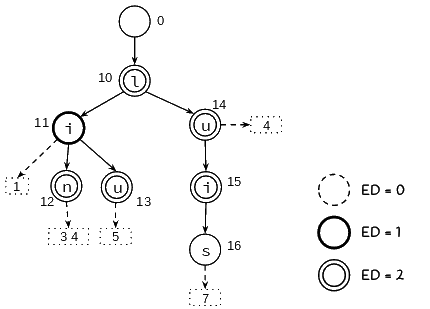
\includegraphics[scale=0.45]{pictures/ican_5.png}
      \centering
    \end{figure}
    
    \textbf{4) query ``nli''}
    
    $\Phi_{p_x} = \big\{ \big \langle 0, 2 \big \rangle, \big \langle 10, 1 \big \rangle, \big \langle 11, 2 \big \rangle, \big \langle 14, 2 \big \rangle \big\}$
    
    $\Phi_{p_{x+1}} = \big\{ \big \langle 10, 2 \big \rangle, \big \langle 11, 1 \big \rangle, \big \langle 12, 2 \big \rangle, \big \langle 13, 2 \big \rangle, \big \langle 14, 2 \big \rangle, \big \langle 15, 2 \big \rangle \big\}$
    
\end{frame}

\begin{frame}{[ICAN] Efficient interactive fuzzy keyword search, 2009}

    \begin{figure}
      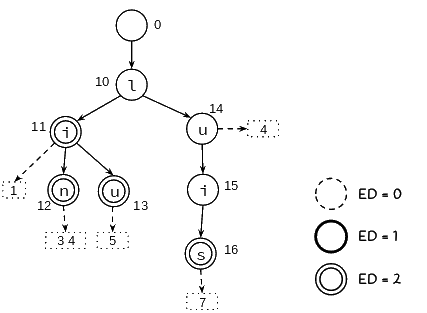
\includegraphics[scale=0.45]{pictures/ican_6.png}
      \centering
    \end{figure}
    
    \textbf{5) query ``nlis''}
    
    $\Phi_{p_{x}} = \big\{ \big \langle 10, 2 \big \rangle, \big \langle 11, 1 \big \rangle, \big \langle 12, 2 \big \rangle, \big \langle 13, 2 \big \rangle, \big \langle 14, 2 \big \rangle, \big \langle 15, 2 \big \rangle \big\}$
    
    $\Phi_{p_{x+1}} = \big\{ \big \langle 11, 1 \big \rangle, \big \langle 12, 2 \big \rangle, \big \langle 13, 2 \big \rangle, \big \langle 16, 2 \big \rangle \big\}$
    
\end{frame}

\begin{frame}{[ICAN] Efficient interactive fuzzy keyword search, 2009}

    Experimentos:

    \begin{figure}
      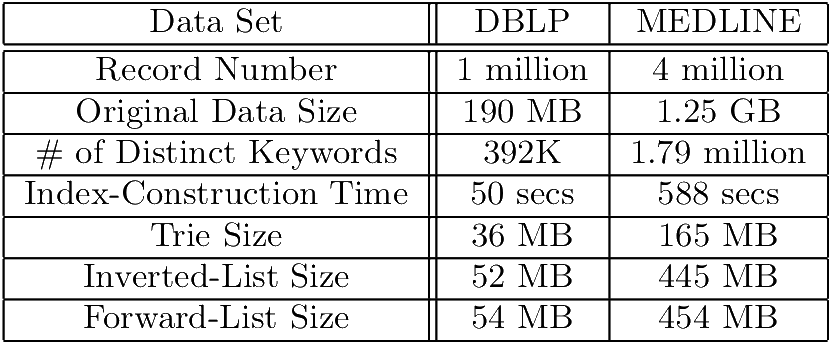
\includegraphics[scale=0.33]{pictures/icpan_2_ex.png}
      \centering
    \end{figure}
    
\end{frame}

\begin{frame}{[ICAN] Efficient interactive fuzzy keyword search, 2009}

    Experimentos:

    \begin{figure}
      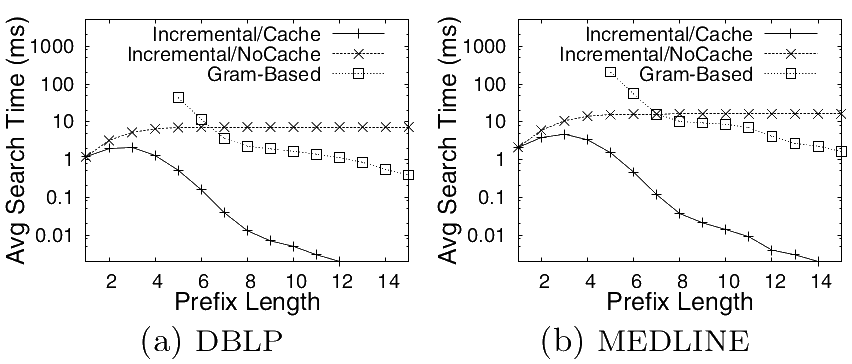
\includegraphics[scale=0.35]{pictures/ican_0_ex.png}
      \centering
    \end{figure}
    
\end{frame}

\begin{frame}{[ICAN] Efficient interactive fuzzy keyword search, 2009}

    Experimentos:

    \begin{figure}
      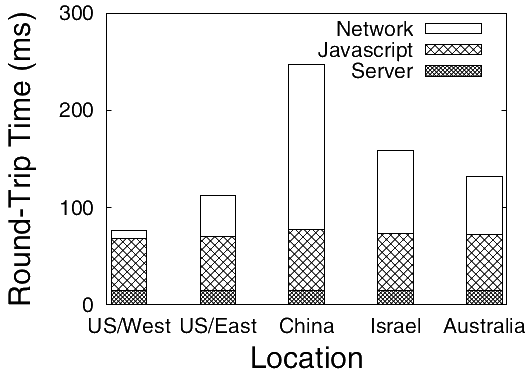
\includegraphics[scale=0.40]{pictures/ican_1_ex.png}
      \centering
    \end{figure}
    
\end{frame}

\subsection{ICPAN}

\begin{frame}{[ICPAN] Efficient fuzzy full-text type-ahead search, \cite{IPCAN}}

    \large
    \begin{itemize}
        \item O Algoritmo ICPAN é uma extensão do ICAN;
        \item Utiliza o conceito de nós fundamentais;
    \end{itemize}
    
    São abordados técnicas para \textbf{prefixo único} e \textbf{prefixo com múltiplas palavras}.
    
\end{frame}

\begin{frame}{[ICPAN] Efficient fuzzy full-text type-ahead search, 2011}
    
    Considere a consulta ``nl'' com o limiar $\tau = 2$, onde: \[\Phi_{nl} = \big\{ \big \langle n_{0}, 2 \big \rangle, \big \langle n_{10}, 1 \big \rangle, \big \langle n_{11}, 2 \big \rangle, \big \langle n_{14}, 2 \big \rangle \big\}\]
    
    \begin{figure}
      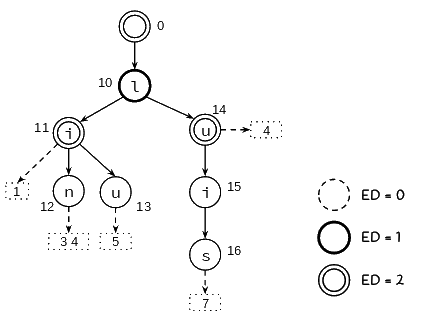
\includegraphics[scale=0.32]{pictures/ican_4.png}
      \centering
    \end{figure}
    
    Apesar de $n_{11}$ (``li'') e $n_{14}$ (``lu'') serem nós ativos, não é necessário guardá-los, assim sendo nós podemos usar o nó ativo $n_{10}$ (``l'') para computar a similaridade das palavras de ``li'' e ``lu'' usando ``l''.
    
\end{frame}

\begin{frame}{[ICPAN] Efficient fuzzy full-text type-ahead search, 2011}

    \large
    Há dois passos para obter $\Phi_{p_{x+1}}$ a partir de $\Phi_{p_{x}}$.

    \begin{enumerate}
        \item $n \in \Phi_{p_{x+1}}$ se $\nexists n_a \mid n_a \in \Phi_{p_{x}} \land \xi_{n} + 1 \le \tau$ então adicionamos $\big \langle n, \xi_{n} + 1 \big \rangle$ em $\Phi_{p_{x+1}}$.
        \item $\forall n_d$ descendente de $n$ fazemos uma avaliação utilizando três conceitos. 
    \end{enumerate}
    
\end{frame}

\begin{frame}{[ICPAN] Efficient fuzzy full-text type-ahead search, 2011}
    
    \large
    Conceitos básicos para definir os nós ativos fundamentais descendentes:
    
    \begin{enumerate}
        \item O nó \textit{n} deve ser um nó ativo; \pause
        \item O último caractere do nó ativo \textit{n} deve dar \textit{match} com algum caractere na consulta; \pause
        \item Se não deu \textit{match} deletar o último caractere do nó ativo \textit{n} e verificar se dar \textit{match}. Se sim, seu ancestral (pai) é um nó ativo fundamental. Repetir o passo \textbf{3} caso contrário.
    \end{enumerate}
    
\end{frame}

\begin{frame}{[ICPAN] Efficient fuzzy full-text type-ahead search, 2011}
    
    \small
    Suponhamos que $\tau = 2$. Um usuário digita um prefixo \textit{p} = ``nlis''. Os prefixos ``li'', ``lin'', ``liu'' e ``luis'' são todos similares para \textit{p}. \pause

    \begin{figure}
      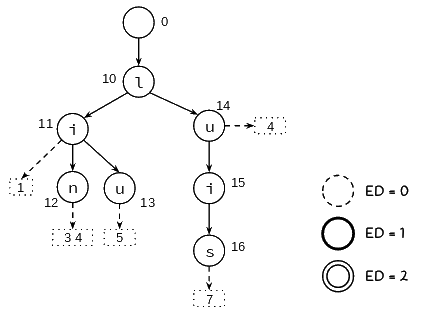
\includegraphics[scale=0.50]{pictures/ipcan_default.png}
      \centering
    \end{figure}
    
\end{frame}

\begin{frame}{[ICPAN] Efficient fuzzy full-text type-ahead search, 2011}
    
    \small
    Suponhamos que $\tau = 2$. Um usuário digita um prefixo \textit{p} = ``nlis''. Os prefixos ``li'', ``lin'', ``liu'' e ``luis'' são todos similares para \textit{p}.

    \begin{figure}
      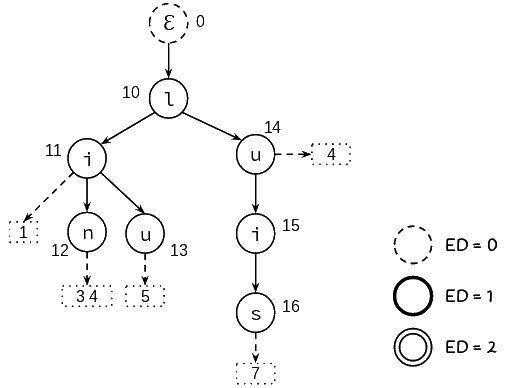
\includegraphics[scale=0.42]{pictures/icpan_1.png}
      \centering
    \end{figure}
    
    \textbf{1) Inicialização}
    
\end{frame}

\begin{frame}{[ICPAN] Efficient fuzzy full-text type-ahead search, 2011}
    
    \small
    Suponhamos que $\tau = 2$. Um usuário digita um prefixo \textit{p} = ``nlis''. Os prefixos ``li'', ``lin'', ``liu'' e ``luis'' são todos similares para \textit{p}.

    \begin{figure}
      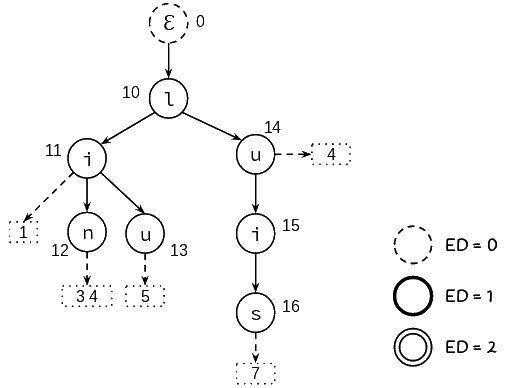
\includegraphics[scale=0.42]{pictures/icpan_1.png}
      \centering
    \end{figure}
    
    \textbf{2) query ``n'' (recupera os nós anteriores)}
    
\end{frame}

\begin{frame}{[ICPAN] Efficient fuzzy full-text type-ahead search, 2011}
    
    \small
    Suponhamos que $\tau = 2$. Um usuário digita um prefixo \textit{p} = ``nlis''. Os prefixos ``li'', ``lin'', ``liu'' e ``luis'' são todos similares para \textit{p}.

    \begin{figure}
      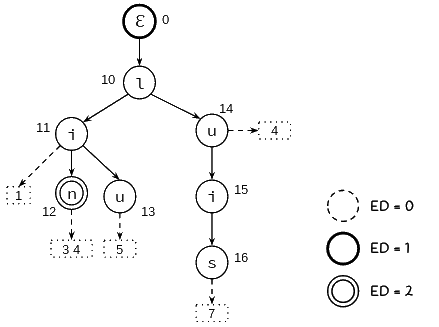
\includegraphics[scale=0.50]{pictures/ipcan_2.png}
      \centering
    \end{figure}
    
    \textbf{2) query ``n'' (calcula os nós ativos fundamentais)}
    
\end{frame}

\begin{frame}{[ICPAN] Efficient fuzzy full-text type-ahead search, 2011}
    
    \small
    Suponhamos que $\tau = 2$. Um usuário digita um prefixo \textit{p} = ``nlis''. Os prefixos ``li'', ``lin'', ``liu'' e ``luis'' são todos similares para \textit{p}.

    \begin{figure}
      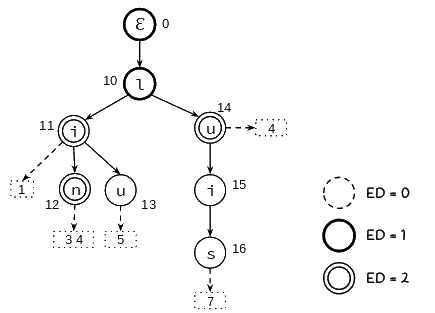
\includegraphics[scale=0.50]{pictures/ipcan_full_1.png}
      \centering
    \end{figure}
    
    \textbf{2) query ``n'' (Recupera todos os nós ativos)}
    
\end{frame}

\begin{frame}{[ICPAN] Efficient fuzzy full-text type-ahead search, 2011}
    
    \small
    Suponhamos que $\tau = 2$. Um usuário digita um prefixo \textit{p} = ``nlis''. Os prefixos ``li'', ``lin'', ``liu'' e ``luis'' são todos similares para \textit{p}.

    \begin{figure}
      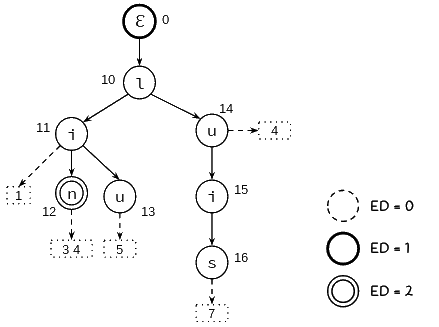
\includegraphics[scale=0.50]{pictures/ipcan_2.png}
      \centering
    \end{figure}
    
    \textbf{2) query ``nl'' (recupera os nós anteriores)}
    
\end{frame}

\begin{frame}{[ICPAN] Efficient fuzzy full-text type-ahead search, 2011}
    
    \small
    Suponhamos que $\tau = 2$. Um usuário digita um prefixo \textit{p} = ``nlis''. Os prefixos ``li'', ``lin'', ``liu'' e ``luis'' são todos similares para \textit{p}.

    \begin{figure}
      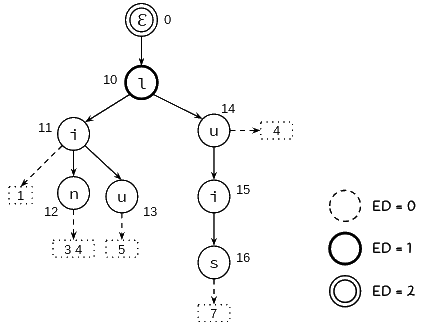
\includegraphics[scale=0.50]{pictures/ipcan_3.png}
      \centering
    \end{figure}
    
    \textbf{2) query ``nl'' (calcula os nós ativos fundamentais)}
    
\end{frame}

\begin{frame}{[ICPAN] Efficient fuzzy full-text type-ahead search, 2011}
    
    \small
    Suponhamos que $\tau = 2$. Um usuário digita um prefixo \textit{p} = ``nlis''. Os prefixos ``li'', ``lin'', ``liu'' e ``luis'' são todos similares para \textit{p}.

    \begin{figure}
      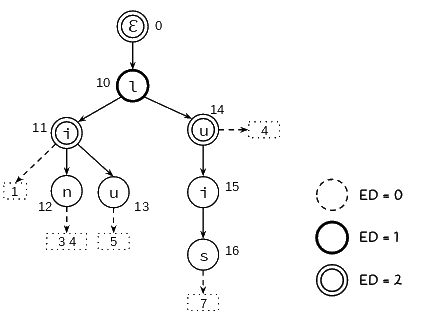
\includegraphics[scale=0.50]{pictures/ipcan_full_2.png}
      \centering
    \end{figure}
    
    \textbf{2) query ``nl'' (Recupera todos os nós ativos)}
    
\end{frame}

\begin{frame}{[ICPAN] Efficient fuzzy full-text type-ahead search, 2011}
    
    \small
    Suponhamos que $\tau = 2$. Um usuário digita um prefixo \textit{p} = ``nlis''. Os prefixos ``li'', ``lin'', ``liu'' e ``luis'' são todos similares para \textit{p}.

    \begin{figure}
      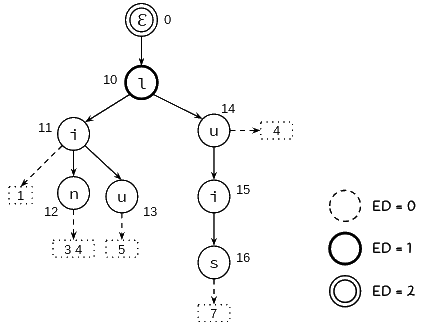
\includegraphics[scale=0.50]{pictures/ipcan_3.png}
      \centering
    \end{figure}
    
    \textbf{2) query ``nli'' (recupera os nós anteriores)}
    
\end{frame}

\begin{frame}{[ICPAN] Efficient fuzzy full-text type-ahead search, 2011}
    
    \small
    Suponhamos que $\tau = 2$. Um usuário digita um prefixo \textit{p} = ``nlis''. Os prefixos ``li'', ``lin'', ``liu'' e ``luis'' são todos similares para \textit{p}.

    \begin{figure}
      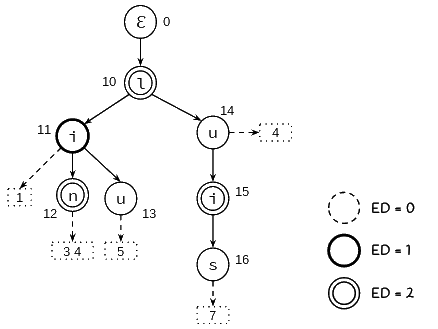
\includegraphics[scale=0.50]{pictures/icpan_4.png}
      \centering
    \end{figure}
    
    \textbf{2) query ``nli'' (calcula os nós ativos fundamentais)}
    
\end{frame}

\begin{frame}{[ICPAN] Efficient fuzzy full-text type-ahead search, 2011}
    
    \small
    Suponhamos que $\tau = 2$. Um usuário digita um prefixo \textit{p} = ``nlis''. Os prefixos ``li'', ``lin'', ``liu'' e ``luis'' são todos similares para \textit{p}.

    \begin{figure}
      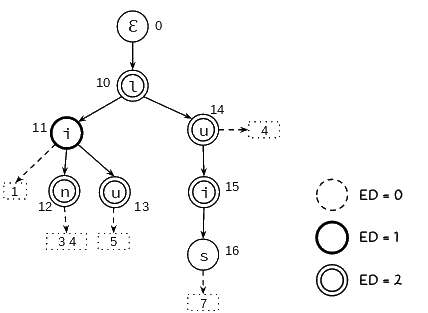
\includegraphics[scale=0.50]{pictures/ipcan_full_3.png}
      \centering
    \end{figure}
    
    \textbf{2) query ``nli'' (Recupera todos os nós ativos)}
    
\end{frame}

\begin{frame}{[ICPAN] Efficient fuzzy full-text type-ahead search, 2011}
    
    \small
    Suponhamos que $\tau = 2$. Um usuário digita um prefixo \textit{p} = ``nlis''. Os prefixos ``li'', ``lin'', ``liu'' e ``luis'' são todos similares para \textit{p}.

    \begin{figure}
      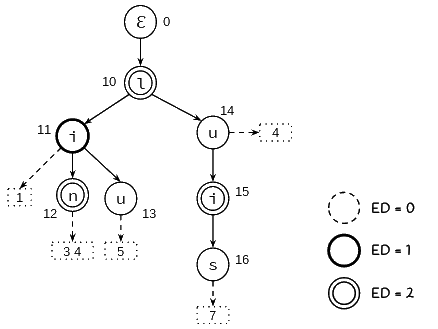
\includegraphics[scale=0.50]{pictures/icpan_4.png}
      \centering
    \end{figure}
    
    \textbf{2) query ``nlis'' (recupera os nós anteriores)}
    
\end{frame}

\begin{frame}{[ICPAN] Efficient fuzzy full-text type-ahead search, 2011}
    
    \small
    Suponhamos que $\tau = 2$. Um usuário digita um prefixo \textit{p} = ``nlis''. Os prefixos ``li'', ``lin'', ``liu'' e ``luis'' são todos similares para \textit{p}.

    \begin{figure}
      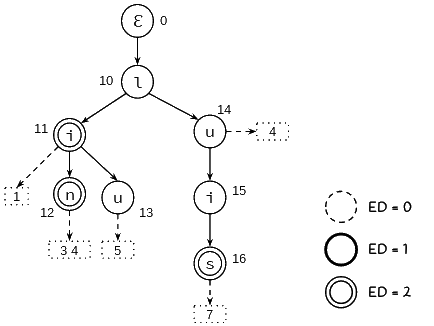
\includegraphics[scale=0.50]{pictures/icpan_5.png}
      \centering
    \end{figure}
    
    \textbf{2) query ``nlis'' (calcula os nós ativos fundamentais)}
    
\end{frame}

\begin{frame}{[ICPAN] Efficient fuzzy full-text type-ahead search, 2011}
    
    \small
    Suponhamos que $\tau = 2$. Um usuário digita um prefixo \textit{p} = ``nlis''. Os prefixos ``li'', ``lin'', ``liu'' e ``luis'' são todos similares para \textit{p}.

    \begin{figure}
      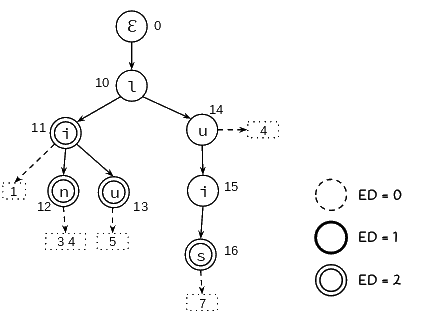
\includegraphics[scale=0.50]{pictures/ipcan_full_4.png}
      \centering
    \end{figure}
    
    \textbf{2) query ``nlis'' (Recupera todos os nós ativos)}
    
\end{frame}

\begin{frame}{[ICPAN] Efficient fuzzy full-text type-ahead search, 2011}
    
    Experimentos:

    \begin{figure}
      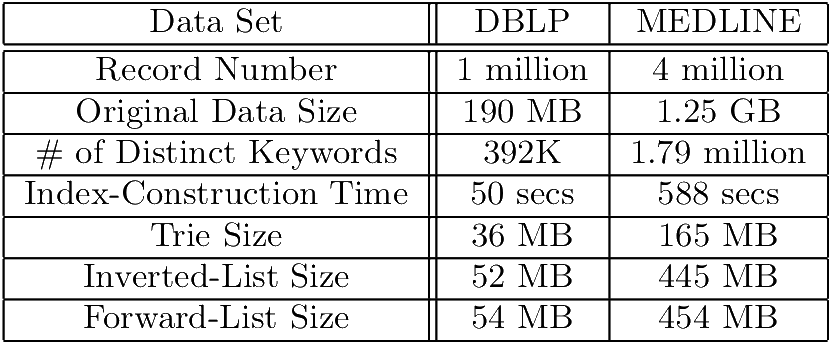
\includegraphics[scale=0.33]{pictures/icpan_2_ex.png}
      \centering
    \end{figure}
    
\end{frame}

\begin{frame}{[ICPAN] Efficient fuzzy full-text type-ahead search, 2011}
    
    Experimentos: Eficiência de busca exata. a) DBLP, b) MEDLINE

    \begin{figure}
      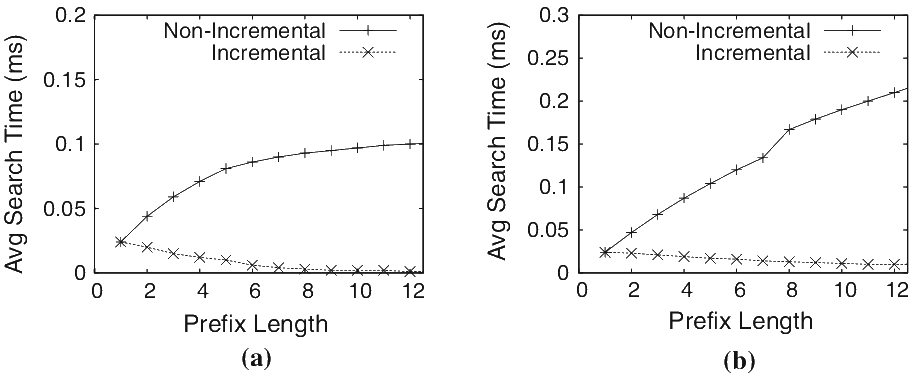
\includegraphics[scale=0.33]{pictures/icpan_3_ex.png}
      \centering
    \end{figure}
    
\end{frame}

\begin{frame}{[ICPAN] Efficient fuzzy full-text type-ahead search, 2011}
    
    Experimentos: Computação de prefixos similares para um palavra-chave ($\tau = 2$). a) DBLP, b) MEDLINE

    \begin{figure}
      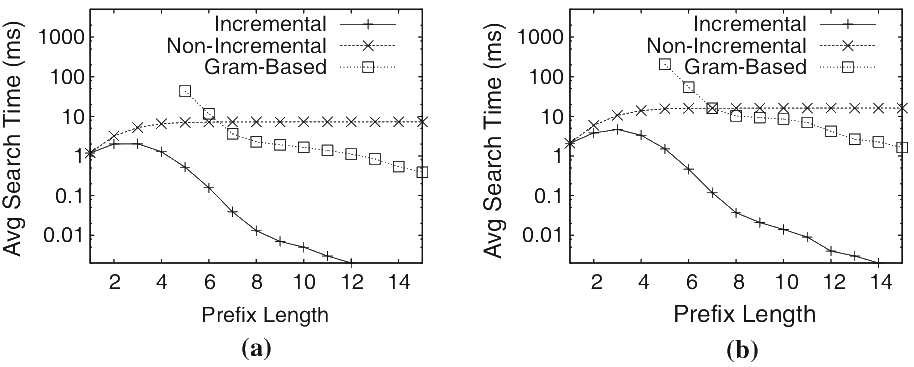
\includegraphics[scale=0.33]{pictures/icpan_4_ex.png}
      \centering
    \end{figure}
    
\end{frame}

\begin{frame}{[ICPAN] Efficient fuzzy full-text type-ahead search, 2011}
    
    Experimentos: Tamanho da memória para computar prefixos similares para uma palavra-chave.

    \begin{figure}
      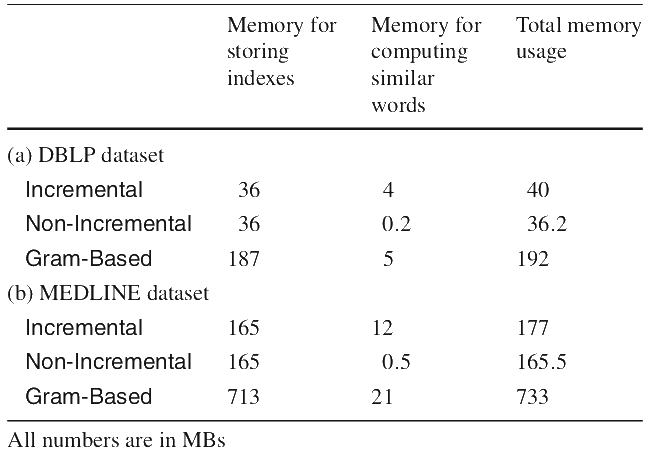
\includegraphics[scale=0.37]{pictures/icpan_5_ex.png}
      \centering
    \end{figure}
    
\end{frame}

\begin{frame}{[ICPAN] Efficient fuzzy full-text type-ahead search, 2011}
    
    Experimentos: Número de nós ativos para uma palavra-chave ($\tau = 3)$. a) DBLP, b) MEDLINE

    \begin{figure}
      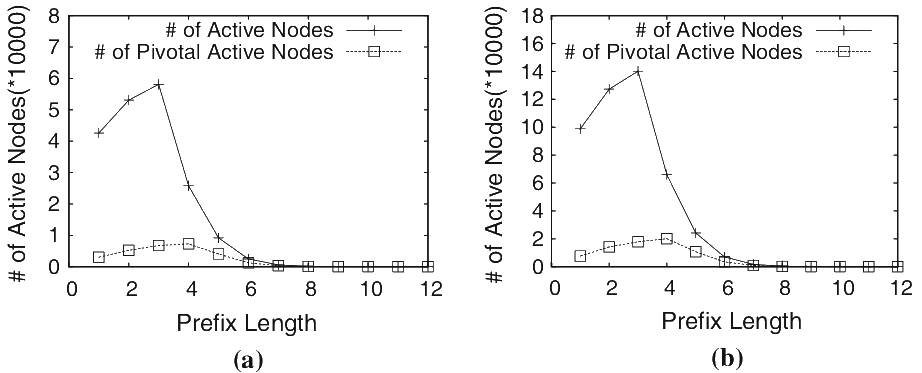
\includegraphics[scale=0.33]{pictures/icpan_6_ex.png}
      \centering
    \end{figure}
    
\end{frame}

\begin{frame}{[ICPAN] Efficient fuzzy full-text type-ahead search, 2011}
    
    Experimentos: Tempo para computar nós ativos para uma palavra-chave ($\tau = 3$). a) DBLP, b) MEDLINE

    \begin{figure}
      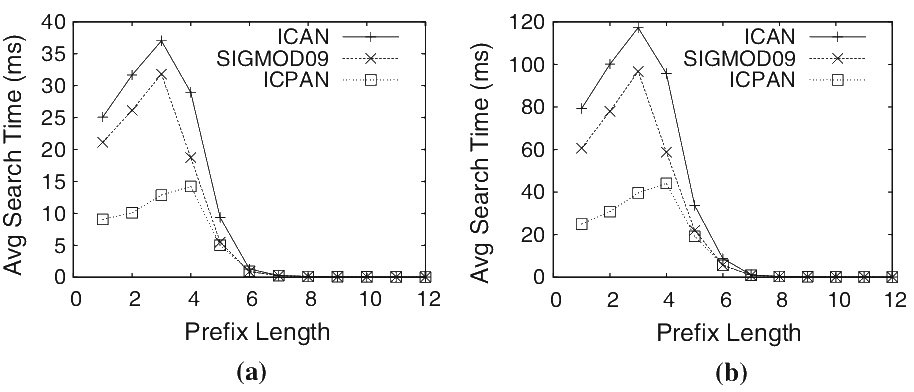
\includegraphics[scale=0.33]{pictures/icpan_7_ex.png}
      \centering
    \end{figure}
    
\end{frame}

\begin{frame}{[ICPAN] Efficient fuzzy full-text type-ahead search, 2011}
    
    Experimentos: Eficiência de consultas de palavras únicas (variando $\tau$). a) DBLP, b) MEDLINE

    \begin{figure}
      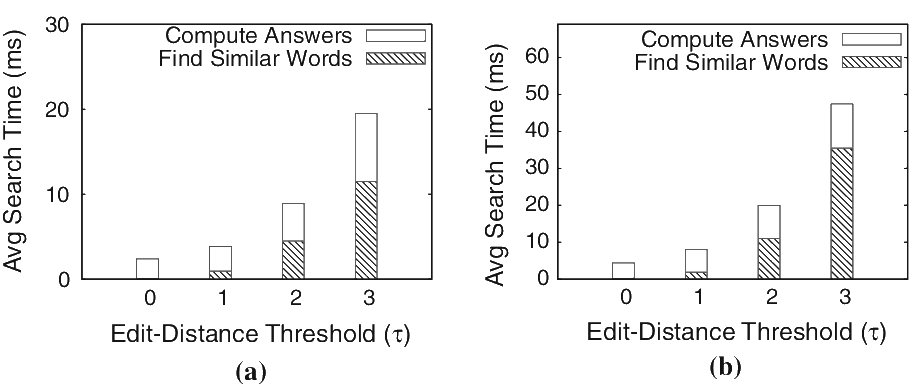
\includegraphics[scale=0.33]{pictures/icpan_8_ex.png}
      \centering
    \end{figure}
    
\end{frame}

\begin{frame}{[ICPAN] Efficient fuzzy full-text type-ahead search, 2011}
    
    Experimentos: Palavras únicas

    \begin{figure}
      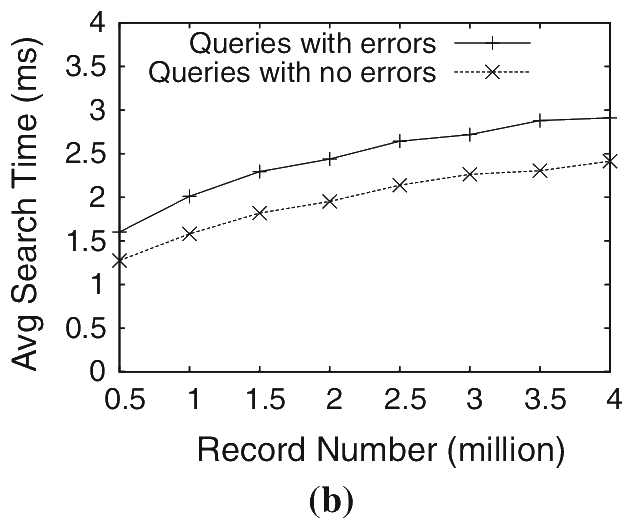
\includegraphics[scale=0.35]{pictures/icpan_9_ex.png}
      \centering
    \end{figure}
    
\end{frame}

\begin{frame}{[ICPAN] Efficient fuzzy full-text type-ahead search, 2011}
    
    Experimentos: Tempo para diferentes localidades

    \begin{figure}
      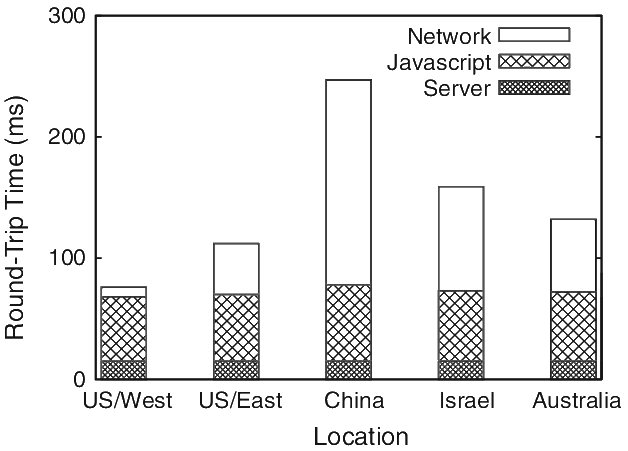
\includegraphics[scale=0.35]{pictures/icpan_10_ex.png}
      \centering
    \end{figure}
    
\end{frame}

\subsection{BEVA}

\begin{frame}{[BEVA] BEVA: An efficient Query Processing algorithm for Error-Tolerant Autocompletion, \cite{BEVA}}

    \large
    Utiliza os conceitos de:
    
    \begin{itemize}
        \item \textbf{Nós de fronteira}. 
        \item \textbf{Vetores de edição}.
        \item \textbf{Autômatos}.
    \end{itemize}
    
    Possui variações, tais como PEVA e UPEVA.
    
\end{frame}

\begin{frame}{[BEVA] BEVA: An efficient Query Processing algorithm for Error-Tolerant Autocompletion, 2016}

    Dado $\mathcal{V}_Q$, o conjunto pode ter dois prefixos $p$ e $p'$ tal que $p' \le p$. Se remover todos os $ps$, é obtido o \textbf{conjunto de nós ativos da fronteira}.
    
    $\mathcal{B}_Q =  \{ p \mid p \in \mathcal{V}_Q \land (\nexists p' \in \mathcal{V}_Q \land p' \le p)\}$ 

    \begin{figure}
      \includegraphics[scale=0.35]{pictures/boundary_active_nodes_beva.png}
      \centering
    \end{figure}
    
\end{frame}

\begin{frame}{[BEVA] BEVA: An efficient Query Processing algorithm for Error-Tolerant Autocompletion, 2016}

    Como computar o limiar de distância de edição ? \pause
    
    Utilizamos \textbf{Algoritmo de programação dinâmica}. \pause 
    
    Os valores das células podem ser computados baseado na seguinte equação: \[ M[i, j] = min(M[i - 1, j - 1] + \delta(d[j], Q[i]), M[i - 1, j] + 1, M[i, j - 1] + 1) \], onde $\delta(x, y) = 0$ se $x = y$, ou 1 caso contrário. E as condições da fronteira são $M[0, j] = j$ e $M[i, 0] = i$.
    
\end{frame}

\begin{frame}{[BEVA] BEVA: An efficient Query Processing algorithm for Error-Tolerant Autocompletion, 2016}

    Computação do limiar de distância de edição:
  
    \begin{table}[]
    \begin{tabular}{llllll}
     &  & \multicolumn{1}{c}{{\color[HTML]{656565} 0}} & \multicolumn{1}{c}{{\color[HTML]{656565} 1}} & \multicolumn{1}{c}{{\color[HTML]{656565} 2}} & \multicolumn{1}{c}{{\color[HTML]{656565} 3}} \\
     &  &  & \textbf{x} & \textbf{a} & \textbf{d} \\ \cline{3-6} 
    {\color[HTML]{656565} 0} & \multicolumn{1}{l|}{} & \multicolumn{1}{l|}{} & \multicolumn{1}{l|}{} & \multicolumn{1}{l|}{} & \multicolumn{1}{l|}{} \\ \cline{3-6} 
    {\color[HTML]{656565} 1} & \multicolumn{1}{l|}{\textbf{a}} & \multicolumn{1}{l|}{} & \multicolumn{1}{l|}{} & \multicolumn{1}{l|}{} & \multicolumn{1}{l|}{} \\ \cline{3-6} 
    {\color[HTML]{656565} 2} & \multicolumn{1}{l|}{\textbf{b}} & \multicolumn{1}{c|}{} & \multicolumn{1}{c|}{} & \multicolumn{1}{c|}{} & \multicolumn{1}{c|}{} \\ \cline{3-6} 
    {\color[HTML]{656565} 3} & \multicolumn{1}{l|}{\textbf{c}} & \multicolumn{1}{l|}{} & \multicolumn{1}{l|}{} & \multicolumn{1}{l|}{} & \multicolumn{1}{l|}{} \\ \cline{3-6} 
    {\color[HTML]{656565} 4} & \multicolumn{1}{l|}{\textbf{d}} & \multicolumn{1}{c|}{} & \multicolumn{1}{c|}{} & \multicolumn{1}{c|}{} & \multicolumn{1}{c|}{} \\ \cline{3-6} 
    \end{tabular}
    \end{table}
    
\end{frame}

\begin{frame}{[BEVA] BEVA: An efficient Query Processing algorithm for Error-Tolerant Autocompletion, 2016}

    Computação do limiar de distância de edição:
  
    \begin{table}[]
    \begin{tabular}{llllll}
     &  & \multicolumn{1}{c}{{\color[HTML]{656565} 0}} & \multicolumn{1}{c}{{\color[HTML]{656565} 1}} & \multicolumn{1}{c}{{\color[HTML]{656565} 2}} & \multicolumn{1}{c}{{\color[HTML]{656565} 3}} \\
     &  &  & \textbf{x} & \textbf{a} & \textbf{d} \\ \cline{3-6} 
    {\color[HTML]{656565} 0} & \multicolumn{1}{l|}{} & \multicolumn{1}{l|}{{\color[HTML]{000000} 0}} & \multicolumn{1}{l|}{{\color[HTML]{000000} 1}} & \multicolumn{1}{l|}{{\color[HTML]{000000} 2}} & \multicolumn{1}{l|}{{\color[HTML]{000000} 3}} \\ \cline{3-6} 
    {\color[HTML]{656565} 1} & \multicolumn{1}{l|}{\textbf{a}} & \multicolumn{1}{l|}{{\color[HTML]{000000} 1}} & \multicolumn{1}{l|}{{\color[HTML]{000000} }} & \multicolumn{1}{l|}{{\color[HTML]{000000} }} & \multicolumn{1}{l|}{{\color[HTML]{000000} }} \\ \cline{3-6} 
    {\color[HTML]{656565} 2} & \multicolumn{1}{l|}{\textbf{b}} & \multicolumn{1}{c|}{{\color[HTML]{000000} 2}} & \multicolumn{1}{c|}{{\color[HTML]{000000} }} & \multicolumn{1}{c|}{{\color[HTML]{000000} }} & \multicolumn{1}{c|}{{\color[HTML]{000000} }} \\ \cline{3-6} 
    {\color[HTML]{656565} 3} & \multicolumn{1}{l|}{\textbf{c}} & \multicolumn{1}{l|}{{\color[HTML]{000000} 3}} & \multicolumn{1}{l|}{{\color[HTML]{000000} }} & \multicolumn{1}{l|}{{\color[HTML]{000000} }} & \multicolumn{1}{l|}{{\color[HTML]{000000} }} \\ \cline{3-6} 
    {\color[HTML]{656565} 4} & \multicolumn{1}{l|}{\textbf{d}} & \multicolumn{1}{c|}{{\color[HTML]{000000} 4}} & \multicolumn{1}{c|}{{\color[HTML]{000000} }} & \multicolumn{1}{c|}{{\color[HTML]{000000} }} & \multicolumn{1}{c|}{{\color[HTML]{000000} }} \\ \cline{3-6} 
    \end{tabular}
    \end{table}
    
    Inicializamos com a seguinte regra: $M[0, j] = j$ e $M[i, 0] = i$
    
\end{frame}

\begin{frame}{[BEVA] BEVA: An efficient Query Processing algorithm for Error-Tolerant Autocompletion, 2016}

    Computação do limiar de distância de edição:
  
    \begin{table}[]
    \begin{tabular}{llllll}
     &  & \multicolumn{1}{c}{{\color[HTML]{656565} 0}} & \multicolumn{1}{c}{{\color[HTML]{656565} 1}} & \multicolumn{1}{c}{{\color[HTML]{656565} 2}} & \multicolumn{1}{c}{{\color[HTML]{656565} 3}} \\
     &  &  & \textbf{x} & \textbf{a} & \textbf{d} \\ \cline{3-6} 
    {\color[HTML]{656565} 0} & \multicolumn{1}{l|}{} & \multicolumn{1}{l|}{{\color[HTML]{000000} 0}} & \multicolumn{1}{l|}{{\color[HTML]{000000} 1}} & \multicolumn{1}{l|}{{\color[HTML]{000000} 2}} & \multicolumn{1}{l|}{{\color[HTML]{000000} 3}} \\ \cline{3-6} 
    {\color[HTML]{656565} 1} & \multicolumn{1}{l|}{\textbf{a}} & \multicolumn{1}{l|}{{\color[HTML]{000000} 1}} & \multicolumn{1}{l|}{{\color[HTML]{000000} ?}} & \multicolumn{1}{l|}{{\color[HTML]{000000} }} & \multicolumn{1}{l|}{{\color[HTML]{000000} }} \\ \cline{3-6} 
    {\color[HTML]{656565} 2} & \multicolumn{1}{l|}{\textbf{b}} & \multicolumn{1}{c|}{{\color[HTML]{000000} 2}} & \multicolumn{1}{c|}{{\color[HTML]{000000} }} & \multicolumn{1}{c|}{{\color[HTML]{000000} }} & \multicolumn{1}{c|}{{\color[HTML]{000000} }} \\ \cline{3-6} 
    {\color[HTML]{656565} 3} & \multicolumn{1}{l|}{\textbf{c}} & \multicolumn{1}{l|}{{\color[HTML]{000000} 3}} & \multicolumn{1}{l|}{{\color[HTML]{000000} }} & \multicolumn{1}{l|}{{\color[HTML]{000000} }} & \multicolumn{1}{l|}{{\color[HTML]{000000} }} \\ \cline{3-6} 
    {\color[HTML]{656565} 4} & \multicolumn{1}{l|}{\textbf{d}} & \multicolumn{1}{c|}{{\color[HTML]{000000} 4}} & \multicolumn{1}{c|}{{\color[HTML]{000000} }} & \multicolumn{1}{c|}{{\color[HTML]{000000} }} & \multicolumn{1}{c|}{{\color[HTML]{000000} }} \\ \cline{3-6} 
    \end{tabular}
    \end{table}
    
     \[ M[i, j] = min(M[i - 1, j - 1] + \delta(d[j], Q[i]), M[i - 1, j] + 1, M[i, j - 1] + 1) \]
    
\end{frame}

\begin{frame}{[BEVA] BEVA: An efficient Query Processing algorithm for Error-Tolerant Autocompletion, 2016}

    Computação do limiar de distância de edição:
  
    \begin{table}[]
    \begin{tabular}{llllll}
     &  & \multicolumn{1}{c}{{\color[HTML]{656565} 0}} & \multicolumn{1}{c}{{\color[HTML]{656565} 1}} & \multicolumn{1}{c}{{\color[HTML]{656565} 2}} & \multicolumn{1}{c}{{\color[HTML]{656565} 3}} \\
     &  &  & \textbf{x} & \textbf{a} & \textbf{d} \\ \cline{3-6} 
    {\color[HTML]{656565} 0} & \multicolumn{1}{l|}{} & \multicolumn{1}{l|}{{\color[HTML]{000000} 0}} & \multicolumn{1}{l|}{{\color[HTML]{000000} 1}} & \multicolumn{1}{l|}{{\color[HTML]{000000} 2}} & \multicolumn{1}{l|}{{\color[HTML]{000000} 3}} \\ \cline{3-6} 
    {\color[HTML]{656565} 1} & \multicolumn{1}{l|}{\textbf{a}} & \multicolumn{1}{l|}{{\color[HTML]{000000} 1}} & \multicolumn{1}{l|}{{\color[HTML]{000000} ?}} & \multicolumn{1}{l|}{{\color[HTML]{000000} }} & \multicolumn{1}{l|}{{\color[HTML]{000000} }} \\ \cline{3-6} 
    {\color[HTML]{656565} 2} & \multicolumn{1}{l|}{\textbf{b}} & \multicolumn{1}{c|}{{\color[HTML]{000000} 2}} & \multicolumn{1}{c|}{{\color[HTML]{000000} }} & \multicolumn{1}{c|}{{\color[HTML]{000000} }} & \multicolumn{1}{c|}{{\color[HTML]{000000} }} \\ \cline{3-6} 
    {\color[HTML]{656565} 3} & \multicolumn{1}{l|}{\textbf{c}} & \multicolumn{1}{l|}{{\color[HTML]{000000} 3}} & \multicolumn{1}{l|}{{\color[HTML]{000000} }} & \multicolumn{1}{l|}{{\color[HTML]{000000} }} & \multicolumn{1}{l|}{{\color[HTML]{000000} }} \\ \cline{3-6} 
    {\color[HTML]{656565} 4} & \multicolumn{1}{l|}{\textbf{d}} & \multicolumn{1}{c|}{{\color[HTML]{000000} 4}} & \multicolumn{1}{c|}{{\color[HTML]{000000} }} & \multicolumn{1}{c|}{{\color[HTML]{000000} }} & \multicolumn{1}{c|}{{\color[HTML]{000000} }} \\ \cline{3-6} 
    \end{tabular}
    \end{table}
    
    \small
    $M[1, 1] = min(M[1 - 1, 1 - 1] + \delta(d[1], Q[1]), M[1 - 1, 1] + 1, M[1, 1 - 1] + 1)$ \pause
    
    $M[1, 1] = min(M[0, 0] + \delta(x, a), M[0, 1] + 1, M[1, 0] + 1)$ \pause
    
    $M[1, 1] = min(1, 2, 2)$ \pause $\to \textbf{1}$
    
\end{frame}

\begin{frame}{[BEVA] BEVA: An efficient Query Processing algorithm for Error-Tolerant Autocompletion, 2016}

    Computação do limiar de distância de edição:
  
    \begin{table}[]
    \begin{tabular}{llllll}
     &  & \multicolumn{1}{c}{{\color[HTML]{656565} 0}} & \multicolumn{1}{c}{{\color[HTML]{656565} 1}} & \multicolumn{1}{c}{{\color[HTML]{656565} 2}} & \multicolumn{1}{c}{{\color[HTML]{656565} 3}} \\
     &  &  & \textbf{x} & \textbf{a} & \textbf{d} \\ \cline{3-6} 
    {\color[HTML]{656565} 0} & \multicolumn{1}{l|}{} & \multicolumn{1}{l|}{{\color[HTML]{000000} 0}} & \multicolumn{1}{l|}{{\color[HTML]{000000} 1}} & \multicolumn{1}{l|}{{\color[HTML]{000000} 2}} & \multicolumn{1}{l|}{{\color[HTML]{000000} 3}} \\ \cline{3-6} 
    {\color[HTML]{656565} 1} & \multicolumn{1}{l|}{\textbf{a}} & \multicolumn{1}{l|}{{\color[HTML]{000000} 1}} & \multicolumn{1}{l|}{{\color[HTML]{000000} 1}} & \multicolumn{1}{l|}{{\color[HTML]{000000} ?}} & \multicolumn{1}{l|}{{\color[HTML]{000000} }} \\ \cline{3-6} 
    {\color[HTML]{656565} 2} & \multicolumn{1}{l|}{\textbf{b}} & \multicolumn{1}{c|}{{\color[HTML]{000000} 2}} & \multicolumn{1}{c|}{{\color[HTML]{000000} }} & \multicolumn{1}{c|}{{\color[HTML]{000000} }} & \multicolumn{1}{c|}{{\color[HTML]{000000} }} \\ \cline{3-6} 
    {\color[HTML]{656565} 3} & \multicolumn{1}{l|}{\textbf{c}} & \multicolumn{1}{l|}{{\color[HTML]{000000} 3}} & \multicolumn{1}{l|}{{\color[HTML]{000000} }} & \multicolumn{1}{l|}{{\color[HTML]{000000} }} & \multicolumn{1}{l|}{{\color[HTML]{000000} }} \\ \cline{3-6} 
    {\color[HTML]{656565} 4} & \multicolumn{1}{l|}{\textbf{d}} & \multicolumn{1}{c|}{{\color[HTML]{000000} 4}} & \multicolumn{1}{c|}{{\color[HTML]{000000} }} & \multicolumn{1}{c|}{{\color[HTML]{000000} }} & \multicolumn{1}{c|}{{\color[HTML]{000000} }} \\ \cline{3-6} 
    \end{tabular}
    \end{table}
    
    \small
    $M[i, j] = min(M[i - 1, j - 1] + \delta(d[j], Q[i]), M[i - 1, j] + 1, M[i, j - 1] + 1)$ \pause
    
    $M[1, 2] = min(1, 3, 2)$ \pause $\to \textbf{1}$
    
\end{frame}

\begin{frame}{[BEVA] BEVA: An efficient Query Processing algorithm for Error-Tolerant Autocompletion, 2016}

    Computação do limiar de distância de edição:
  
    \begin{table}[]
    \begin{tabular}{llllll}
     &  & \multicolumn{1}{c}{{\color[HTML]{656565} 0}} & \multicolumn{1}{c}{{\color[HTML]{656565} 1}} & \multicolumn{1}{c}{{\color[HTML]{656565} 2}} & \multicolumn{1}{c}{{\color[HTML]{656565} 3}} \\
     &  &  & \textbf{x} & \textbf{a} & \textbf{d} \\ \cline{3-6} 
    {\color[HTML]{656565} 0} & \multicolumn{1}{l|}{} & \multicolumn{1}{l|}{{\color[HTML]{000000} 0}} & \multicolumn{1}{l|}{{\color[HTML]{000000} 1}} & \multicolumn{1}{l|}{{\color[HTML]{000000} 2}} & \multicolumn{1}{l|}{{\color[HTML]{000000} 3}} \\ \cline{3-6} 
    {\color[HTML]{656565} 1} & \multicolumn{1}{l|}{\textbf{a}} & \multicolumn{1}{l|}{{\color[HTML]{000000} 1}} & \multicolumn{1}{l|}{{\color[HTML]{000000} 1}} & \multicolumn{1}{l|}{{\color[HTML]{000000} 1}} & \multicolumn{1}{l|}{{\color[HTML]{000000} ?}} \\ \cline{3-6} 
    {\color[HTML]{656565} 2} & \multicolumn{1}{l|}{\textbf{b}} & \multicolumn{1}{c|}{{\color[HTML]{000000} 2}} & \multicolumn{1}{c|}{{\color[HTML]{000000} }} & \multicolumn{1}{c|}{{\color[HTML]{000000} }} & \multicolumn{1}{c|}{{\color[HTML]{000000} }} \\ \cline{3-6} 
    {\color[HTML]{656565} 3} & \multicolumn{1}{l|}{\textbf{c}} & \multicolumn{1}{l|}{{\color[HTML]{000000} 3}} & \multicolumn{1}{l|}{{\color[HTML]{000000} }} & \multicolumn{1}{l|}{{\color[HTML]{000000} }} & \multicolumn{1}{l|}{{\color[HTML]{000000} }} \\ \cline{3-6} 
    {\color[HTML]{656565} 4} & \multicolumn{1}{l|}{\textbf{d}} & \multicolumn{1}{c|}{{\color[HTML]{000000} 4}} & \multicolumn{1}{c|}{{\color[HTML]{000000} }} & \multicolumn{1}{c|}{{\color[HTML]{000000} }} & \multicolumn{1}{c|}{{\color[HTML]{000000} }} \\ \cline{3-6} 
    \end{tabular}
    \end{table}
    
    \small
    $M[i, j] = min(M[i - 1, j - 1] + \delta(d[j], Q[i]), M[i - 1, j] + 1, M[i, j - 1] + 1)$ \pause
    
    $M[1, 3] = min(3, 4, 2)$ \pause $\to \textbf{2}$
    
\end{frame}

\begin{frame}{[BEVA] BEVA: An efficient Query Processing algorithm for Error-Tolerant Autocompletion, 2016}

    Computação do limiar de distância de edição:
  
    \begin{table}[]
    \begin{tabular}{llllll}
     &  & \multicolumn{1}{c}{{\color[HTML]{656565} 0}} & \multicolumn{1}{c}{{\color[HTML]{656565} 1}} & \multicolumn{1}{c}{{\color[HTML]{656565} 2}} & \multicolumn{1}{c}{{\color[HTML]{656565} 3}} \\
     &  &  & \textbf{x} & \textbf{a} & \textbf{d} \\ \cline{3-6} 
    {\color[HTML]{656565} 0} & \multicolumn{1}{l|}{} & \multicolumn{1}{l|}{{\color[HTML]{000000} 0}} & \multicolumn{1}{l|}{{\color[HTML]{000000} 1}} & \multicolumn{1}{l|}{{\color[HTML]{000000} 2}} & \multicolumn{1}{l|}{{\color[HTML]{000000} 3}} \\ \cline{3-6} 
    {\color[HTML]{656565} 1} & \multicolumn{1}{l|}{\textbf{a}} & \multicolumn{1}{l|}{{\color[HTML]{000000} 1}} & \multicolumn{1}{l|}{{\color[HTML]{000000} 1}} & \multicolumn{1}{l|}{{\color[HTML]{000000} 1}} & \multicolumn{1}{l|}{{\color[HTML]{000000} 2}} \\ \cline{3-6} 
    {\color[HTML]{656565} 2} & \multicolumn{1}{l|}{\textbf{b}} & \multicolumn{1}{c|}{{\color[HTML]{000000} 2}} & \multicolumn{1}{c|}{{\color[HTML]{000000} }} & \multicolumn{1}{c|}{{\color[HTML]{000000} }} & \multicolumn{1}{c|}{{\color[HTML]{000000} }} \\ \cline{3-6} 
    {\color[HTML]{656565} 3} & \multicolumn{1}{l|}{\textbf{c}} & \multicolumn{1}{l|}{{\color[HTML]{000000} 3}} & \multicolumn{1}{l|}{{\color[HTML]{000000} }} & \multicolumn{1}{l|}{{\color[HTML]{000000} }} & \multicolumn{1}{l|}{{\color[HTML]{000000} }} \\ \cline{3-6} 
    {\color[HTML]{656565} 4} & \multicolumn{1}{l|}{\textbf{d}} & \multicolumn{1}{c|}{{\color[HTML]{000000} 4}} & \multicolumn{1}{c|}{{\color[HTML]{000000} }} & \multicolumn{1}{c|}{{\color[HTML]{000000} }} & \multicolumn{1}{c|}{{\color[HTML]{000000} }} \\ \cline{3-6} 
    \end{tabular}
    \end{table}
    
\end{frame}

\begin{frame}{[BEVA] BEVA: An efficient Query Processing algorithm for Error-Tolerant Autocompletion, 2016}

    Computação do limiar de distância de edição:
  
    \begin{table}[]
    \begin{tabular}{llllll}
     &  & \multicolumn{1}{c}{{\color[HTML]{656565} 0}} & \multicolumn{1}{c}{{\color[HTML]{656565} 1}} & \multicolumn{1}{c}{{\color[HTML]{656565} 2}} & \multicolumn{1}{c}{{\color[HTML]{656565} 3}} \\
     &  &  & \textbf{x} & \textbf{a} & \textbf{d} \\ \cline{3-6} 
    {\color[HTML]{656565} 0} & \multicolumn{1}{l|}{} & \multicolumn{1}{l|}{{\color[HTML]{000000} 0}} & \multicolumn{1}{l|}{{\color[HTML]{000000} 1}} & \multicolumn{1}{l|}{{\color[HTML]{000000} 2}} & \multicolumn{1}{l|}{{\color[HTML]{000000} 3}} \\ \cline{3-6} 
    {\color[HTML]{656565} 1} & \multicolumn{1}{l|}{\textbf{a}} & \multicolumn{1}{l|}{{\color[HTML]{000000} 1}} & \multicolumn{1}{l|}{{\color[HTML]{000000} 1}} & \multicolumn{1}{l|}{{\color[HTML]{000000} 1}} & \multicolumn{1}{l|}{{\color[HTML]{000000} 2}} \\ \cline{3-6} 
    {\color[HTML]{656565} 2} & \multicolumn{1}{l|}{\textbf{b}} & \multicolumn{1}{c|}{{\color[HTML]{000000} 2}} & \multicolumn{1}{c|}{{\color[HTML]{000000} 2}} & \multicolumn{1}{c|}{{\color[HTML]{000000} 2}} & \multicolumn{1}{c|}{{\color[HTML]{000000} 2}} \\ \cline{3-6} 
    {\color[HTML]{656565} 3} & \multicolumn{1}{l|}{\textbf{c}} & \multicolumn{1}{l|}{{\color[HTML]{000000} 3}} & \multicolumn{1}{l|}{{\color[HTML]{000000} 3}} & \multicolumn{1}{l|}{{\color[HTML]{000000} 3}} & \multicolumn{1}{l|}{{\color[HTML]{000000} 3}} \\ \cline{3-6} 
    {\color[HTML]{656565} 4} & \multicolumn{1}{l|}{\textbf{d}} & \multicolumn{1}{c|}{{\color[HTML]{000000} 4}} & \multicolumn{1}{c|}{{\color[HTML]{000000} 4}} & \multicolumn{1}{c|}{{\color[HTML]{000000} 4}} & \multicolumn{1}{c|}{{\color[HTML]{000000} 3}} \\ \cline{3-6} 
    \end{tabular}
    \end{table}
    
    $O(n \cdot m)$, onde $n$ e $m$ são os tamanhos de $d$ e $q$, respectivamente.
    
\end{frame}

\begin{frame}{[BEVA] BEVA: An efficient Query Processing algorithm for Error-Tolerant Autocompletion, 2016}

    Definimos a k-diagonal na matriz M tal que $j - i = k$. Para determinar $ed(d, Q) \le \tau$, o \textit{algoritmo de distância de edição} em Ukkonen [1985a] apenas necessita computar as k-diagonais na matriz, onde $k \in [-\tau, \tau]$.
  
    \begin{table}[]
    \begin{tabular}{llllll}
     &  & \multicolumn{1}{c}{{\color[HTML]{656565} 0}} & \multicolumn{1}{c}{{\color[HTML]{656565} 1}} & \multicolumn{1}{c}{{\color[HTML]{656565} 2}} & \multicolumn{1}{c}{{\color[HTML]{656565} 3}} \\
     &  &  & \textbf{x} & \textbf{a} & \textbf{d} \\ \cline{3-6} 
    {\color[HTML]{656565} 0} & \multicolumn{1}{l|}{} & \multicolumn{1}{l|}{{\color[HTML]{000000} 0}} & \multicolumn{1}{l|}{{\color[HTML]{000000} 1}} & \multicolumn{1}{l|}{{\color[HTML]{000000} 2}} & \multicolumn{1}{l|}{{\color[HTML]{000000} 3}} \\ \cline{3-6} 
    {\color[HTML]{656565} 1} & \multicolumn{1}{l|}{\textbf{a}} & \multicolumn{1}{l|}{{\color[HTML]{000000} 1}} & \multicolumn{1}{l|}{{\color[HTML]{000000} 1}} & \multicolumn{1}{l|}{{\color[HTML]{000000} 1}} & \multicolumn{1}{l|}{{\color[HTML]{000000} 2}} \\ \cline{3-6} 
    {\color[HTML]{656565} 2} & \multicolumn{1}{l|}{\textbf{b}} & \multicolumn{1}{c|}{{\color[HTML]{000000} 2}} & \multicolumn{1}{c|}{{\color[HTML]{000000} 2}} & \multicolumn{1}{c|}{{\color[HTML]{000000} 2}} & \multicolumn{1}{c|}{{\color[HTML]{000000} 2}} \\ \cline{3-6} 
    {\color[HTML]{656565} 3} & \multicolumn{1}{l|}{\textbf{c}} & \multicolumn{1}{l|}{{\color[HTML]{000000} 3}} & \multicolumn{1}{l|}{{\color[HTML]{000000} 3}} & \multicolumn{1}{l|}{{\color[HTML]{000000} 3}} & \multicolumn{1}{l|}{{\color[HTML]{000000} 3}} \\ \cline{3-6} 
    {\color[HTML]{656565} 4} & \multicolumn{1}{l|}{\textbf{d}} & \multicolumn{1}{c|}{{\color[HTML]{000000} 4}} & \multicolumn{1}{c|}{{\color[HTML]{000000} 4}} & \multicolumn{1}{c|}{{\color[HTML]{000000} 4}} & \multicolumn{1}{c|}{{\color[HTML]{000000} 3}} \\ \cline{3-6} 
    \end{tabular}
    \end{table}
    
\end{frame}

\begin{frame}{[BEVA] BEVA: An efficient Query Processing algorithm for Error-Tolerant Autocompletion, 2016}

    Definimos a k-diagonal na matriz M tal que $j - i = k$. Para determinar $ed(d, Q) \le \tau$, o \textit{algoritmo de distância de edição} em Ukkonen [1985a] apenas necessita computar as k-diagonais na matriz, onde $k \in [-\tau, \tau]$.
  
    \begin{table}[]
    \begin{tabular}{llllll}
     &  & \multicolumn{1}{c}{{\color[HTML]{656565} 0}} & \multicolumn{1}{c}{{\color[HTML]{656565} 1}} & \multicolumn{1}{c}{{\color[HTML]{656565} 2}} & \multicolumn{1}{c}{{\color[HTML]{656565} 3}} \\
     &  &  & \textbf{x} & \textbf{a} & \textbf{d} \\ \cline{3-6} 
    {\color[HTML]{656565} 0} & \multicolumn{1}{l|}{} & \multicolumn{1}{l|}{\cellcolor[HTML]{656565}{\color[HTML]{000000} 0}} & \multicolumn{1}{l|}{\cellcolor[HTML]{9B9B9B}{\color[HTML]{000000} 1}} & \multicolumn{1}{l|}{{\color[HTML]{000000} 2}} & \multicolumn{1}{l|}{{\color[HTML]{000000} 3}} \\ \cline{3-6} 
    {\color[HTML]{656565} 1} & \multicolumn{1}{l|}{\textbf{a}} & \multicolumn{1}{l|}{\cellcolor[HTML]{9B9B9B}{\color[HTML]{000000} 1}} & \multicolumn{1}{l|}{\cellcolor[HTML]{656565}{\color[HTML]{000000} 1}} & \multicolumn{1}{l|}{\cellcolor[HTML]{9B9B9B}{\color[HTML]{000000} 1}} & \multicolumn{1}{l|}{{\color[HTML]{000000} 2}} \\ \cline{3-6} 
    {\color[HTML]{656565} 2} & \multicolumn{1}{l|}{\textbf{b}} & \multicolumn{1}{c|}{{\color[HTML]{000000} 2}} & \multicolumn{1}{c|}{\cellcolor[HTML]{9B9B9B}{\color[HTML]{000000} 2}} & \multicolumn{1}{c|}{\cellcolor[HTML]{656565}{\color[HTML]{000000} 2}} & \multicolumn{1}{c|}{\cellcolor[HTML]{9B9B9B}{\color[HTML]{000000} 2}} \\ \cline{3-6} 
    {\color[HTML]{656565} 3} & \multicolumn{1}{l|}{\textbf{c}} & \multicolumn{1}{l|}{{\color[HTML]{000000} 3}} & \multicolumn{1}{l|}{{\color[HTML]{000000} 3}} & \multicolumn{1}{l|}{\cellcolor[HTML]{9B9B9B}{\color[HTML]{000000} 3}} & \multicolumn{1}{l|}{\cellcolor[HTML]{656565}{\color[HTML]{000000} 3}} \\ \cline{3-6} 
    {\color[HTML]{656565} 4} & \multicolumn{1}{l|}{\textbf{d}} & \multicolumn{1}{c|}{{\color[HTML]{000000} 4}} & \multicolumn{1}{c|}{{\color[HTML]{000000} 4}} & \multicolumn{1}{c|}{{\color[HTML]{000000} 4}} & \multicolumn{1}{c|}{\cellcolor[HTML]{9B9B9B}{\color[HTML]{000000} 3}} \\ \cline{3-6} 
    \end{tabular}
    \end{table}
    
    Para $\tau = 1$.
    
\end{frame}

\begin{frame}{[BEVA] BEVA: An efficient Query Processing algorithm for Error-Tolerant Autocompletion, 2016}

    \begin{itemize}
        \item A ideia chave do algoritmo \textbf{BEVA} é guardar todas as distâncias de edição entre as $k$-diagonais onde $k \in [-\tau, \tau]$.
        \item Assim, surge a ideia de \textbf{vetor de edição} que mais tarde poderá ser codificado como um estado em um \textit{autômato de vetor de edição}. 
    \end{itemize}

\end{frame}

\begin{frame}{[BEVA] BEVA: An efficient Query Processing algorithm for Error-Tolerant Autocompletion, 2016}

    Suponha $\tau = 1$, Q=``abcd'' e a palavra dado ``xad''. O cálculo dos vetores de edição cru é feito da seguinte forma:
  
    \begin{table}[]
    \begin{tabular}{llllll}
     &  & \multicolumn{1}{c}{{\color[HTML]{656565} 0}} & \multicolumn{1}{c}{{\color[HTML]{656565} 1}} & \multicolumn{1}{c}{{\color[HTML]{656565} 3}} & \multicolumn{1}{c}{{\color[HTML]{656565} 4}} \\
     &  &  & \textbf{x} & \textbf{a} & \textbf{d} \\ \cline{3-6} 
    {\color[HTML]{656565} 0} & \multicolumn{1}{l|}{} & \multicolumn{1}{l|}{\cellcolor[HTML]{009901}{\color[HTML]{000000} 0}} & \multicolumn{1}{l|}{\cellcolor[HTML]{F8FF00}{\color[HTML]{000000} 1}} & \multicolumn{1}{l|}{{\color[HTML]{000000} 2}} & \multicolumn{1}{l|}{{\color[HTML]{000000} 3}} \\ \cline{3-6} 
    {\color[HTML]{656565} 1} & \multicolumn{1}{l|}{\textbf{a}} & \multicolumn{1}{l|}{\cellcolor[HTML]{009901}{\color[HTML]{000000} 1}} & \multicolumn{1}{l|}{\cellcolor[HTML]{F8FF00}{\color[HTML]{000000} 1}} & \multicolumn{1}{l|}{\cellcolor[HTML]{009901}{\color[HTML]{000000} 1}} & \multicolumn{1}{l|}{{\color[HTML]{000000} 2}} \\ \cline{3-6} 
    {\color[HTML]{656565} 2} & \multicolumn{1}{l|}{\textbf{b}} & \multicolumn{1}{c|}{{\color[HTML]{000000} 2}} & \multicolumn{1}{c|}{\cellcolor[HTML]{F8FF00}{\color[HTML]{000000} 2}} & \multicolumn{1}{c|}{\cellcolor[HTML]{009901}{\color[HTML]{000000} 2}} & \multicolumn{1}{c|}{\cellcolor[HTML]{F8FF00}{\color[HTML]{000000} 2}} \\ \cline{3-6} 
    {\color[HTML]{656565} 3} & \multicolumn{1}{l|}{\textbf{c}} & \multicolumn{1}{l|}{{\color[HTML]{000000} 3}} & \multicolumn{1}{l|}{{\color[HTML]{000000} 3}} & \multicolumn{1}{l|}{\cellcolor[HTML]{009901}{\color[HTML]{000000} 3}} & \multicolumn{1}{l|}{\cellcolor[HTML]{F8FF00}{\color[HTML]{000000} 3}} \\ \cline{3-6} 
    {\color[HTML]{656565} 4} & \multicolumn{1}{l|}{\textbf{d}} & \multicolumn{1}{c|}{{\color[HTML]{000000} 4}} & \multicolumn{1}{c|}{{\color[HTML]{000000} 4}} & \multicolumn{1}{c|}{{\color[HTML]{000000} 4}} & \multicolumn{1}{c|}{\cellcolor[HTML]{F8FF00}{\color[HTML]{000000} 3}} \\ \cline{3-6} 
    \end{tabular}
    \end{table} 
    
\end{frame}

\begin{frame}{[BEVA] BEVA: An efficient Query Processing algorithm for Error-Tolerant Autocompletion, 2016}

    \begin{itemize}
        \item Não é guardado valores que sejam maior que $\tau$. 
        \item Assim sendo, é substituído os valores dessas células para um símbolo especial $\#$ para gerar o vetor de edição. 
    \end{itemize}
    \pause
  
    \begin{table}[]
    \begin{tabular}{llllll}
     &  & \multicolumn{1}{c}{{\color[HTML]{656565} 0}} & \multicolumn{1}{c}{{\color[HTML]{656565} 1}} & \multicolumn{1}{c}{{\color[HTML]{656565} 3}} & \multicolumn{1}{c}{{\color[HTML]{656565} 4}} \\ \cline{3-3}
     & \multicolumn{1}{l|}{} & \multicolumn{1}{l|}{\cellcolor[HTML]{009901}1} & \textbf{x} & \textbf{a} & \textbf{d} \\ \cline{3-6} 
    {\color[HTML]{656565} 0} & \multicolumn{1}{l|}{} & \multicolumn{1}{l|}{\cellcolor[HTML]{009901}{\color[HTML]{000000} 0}} & \multicolumn{1}{l|}{\cellcolor[HTML]{F8FF00}{\color[HTML]{000000} 1}} & \multicolumn{1}{l|}{{\color[HTML]{000000} }} & \multicolumn{1}{l|}{{\color[HTML]{000000} }} \\ \cline{3-6} 
    {\color[HTML]{656565} 1} & \multicolumn{1}{l|}{\textbf{a}} & \multicolumn{1}{l|}{\cellcolor[HTML]{009901}{\color[HTML]{000000} 1}} & \multicolumn{1}{l|}{\cellcolor[HTML]{F8FF00}{\color[HTML]{000000} 1}} & \multicolumn{1}{l|}{\cellcolor[HTML]{009901}{\color[HTML]{000000} 1}} & \multicolumn{1}{l|}{{\color[HTML]{000000} }} \\ \cline{3-6} 
    {\color[HTML]{656565} 2} & \multicolumn{1}{l|}{\textbf{b}} & \multicolumn{1}{c|}{{\color[HTML]{000000} }} & \multicolumn{1}{c|}{\cellcolor[HTML]{F8FF00}{\color[HTML]{000000} $\#$}} & \multicolumn{1}{c|}{\cellcolor[HTML]{009901}{\color[HTML]{000000} $\#$}} & \multicolumn{1}{c|}{\cellcolor[HTML]{F8FF00}{\color[HTML]{000000} $\#$}} \\ \cline{3-6} 
    {\color[HTML]{656565} 3} & \multicolumn{1}{l|}{\textbf{c}} & \multicolumn{1}{l|}{{\color[HTML]{000000} }} & \multicolumn{1}{l|}{{\color[HTML]{000000} }} & \multicolumn{1}{l|}{\cellcolor[HTML]{009901}{\color[HTML]{000000} $\#$}} & \multicolumn{1}{l|}{\cellcolor[HTML]{F8FF00}{\color[HTML]{000000} $\#$}} \\ \cline{3-6} 
    {\color[HTML]{656565} 4} & \multicolumn{1}{l|}{\textbf{d}} & \multicolumn{1}{c|}{{\color[HTML]{000000} }} & \multicolumn{1}{c|}{{\color[HTML]{000000} }} & \multicolumn{1}{c|}{{\color[HTML]{000000} }} & \multicolumn{1}{c|}{\cellcolor[HTML]{F8FF00}{\color[HTML]{000000} $\#$}} \\ \cline{3-6} 
     &  & $V_0$ & $V_1$ & $V_2$ & $V_3$
    \end{tabular}
    \end{table}
   
\end{frame}

\begin{frame}{[BEVA] BEVA: An efficient Query Processing algorithm for Error-Tolerant Autocompletion, 2016}

    \small
    \begin{itemize}
        \item O vetor de edição da coluna 0 sempre tem a forma $[\underbrace{\tau, \tau - 1, \ldots, 1}_{\tau}, 0, \underbrace
{1, 2, \ldots, \tau}_{\tau}]$, pois a palavra na coluna 0 é vazia. Tal característica é nomeada como \textbf{vetor de edição inicial}.
        \item Similarmente, o vetor com todo os símbolos $\#$, que é, $[\underbrace{\#, \#, \ldots, \#}_{2\tau + 1}]$ é nomeado como \textbf{vetor de edição final}.
    \end{itemize}

    \begin{table}[]
    \begin{tabular}{llllll}
     &  & \multicolumn{1}{c}{{\color[HTML]{656565} 0}} & \multicolumn{1}{c}{{\color[HTML]{656565} 1}} & \multicolumn{1}{c}{{\color[HTML]{656565} 3}} & \multicolumn{1}{c}{{\color[HTML]{656565} 4}} \\ \cline{3-3}
     & \multicolumn{1}{l|}{} & \multicolumn{1}{l|}{\cellcolor[HTML]{009901}1} & \textbf{x} & \textbf{a} & \textbf{d} \\ \cline{3-6} 
    {\color[HTML]{656565} 0} & \multicolumn{1}{l|}{} & \multicolumn{1}{l|}{\cellcolor[HTML]{009901}{\color[HTML]{000000} 0}} & \multicolumn{1}{l|}{\cellcolor[HTML]{F8FF00}{\color[HTML]{000000} 1}} & \multicolumn{1}{l|}{{\color[HTML]{000000} }} & \multicolumn{1}{l|}{{\color[HTML]{000000} }} \\ \cline{3-6} 
    {\color[HTML]{656565} 1} & \multicolumn{1}{l|}{\textbf{a}} & \multicolumn{1}{l|}{\cellcolor[HTML]{009901}{\color[HTML]{000000} 1}} & \multicolumn{1}{l|}{\cellcolor[HTML]{F8FF00}{\color[HTML]{000000} 1}} & \multicolumn{1}{l|}{\cellcolor[HTML]{009901}{\color[HTML]{000000} 1}} & \multicolumn{1}{l|}{{\color[HTML]{000000} }} \\ \cline{3-6} 
    {\color[HTML]{656565} 2} & \multicolumn{1}{l|}{\textbf{b}} & \multicolumn{1}{c|}{{\color[HTML]{000000} }} & \multicolumn{1}{c|}{\cellcolor[HTML]{F8FF00}{\color[HTML]{000000} $\#$}} & \multicolumn{1}{c|}{\cellcolor[HTML]{009901}{\color[HTML]{000000} $\#$}} & \multicolumn{1}{c|}{\cellcolor[HTML]{F8FF00}{\color[HTML]{000000} $\#$}} \\ \cline{3-6} 
    {\color[HTML]{656565} 3} & \multicolumn{1}{l|}{\textbf{c}} & \multicolumn{1}{l|}{{\color[HTML]{000000} }} & \multicolumn{1}{l|}{{\color[HTML]{000000} }} & \multicolumn{1}{l|}{\cellcolor[HTML]{009901}{\color[HTML]{000000} $\#$}} & \multicolumn{1}{l|}{\cellcolor[HTML]{F8FF00}{\color[HTML]{000000} $\#$}} \\ \cline{3-6} 
    {\color[HTML]{656565} 4} & \multicolumn{1}{l|}{\textbf{d}} & \multicolumn{1}{c|}{{\color[HTML]{000000} }} & \multicolumn{1}{c|}{{\color[HTML]{000000} }} & \multicolumn{1}{c|}{{\color[HTML]{000000} }} & \multicolumn{1}{c|}{\cellcolor[HTML]{F8FF00}{\color[HTML]{000000} $\#$}} \\ \cline{3-6} 
    \end{tabular}
    \end{table}
   
\end{frame}

\begin{frame}{[BEVA] BEVA: An efficient Query Processing algorithm for Error-Tolerant Autocompletion, 2016}

    Função de transição $= f(v_j, \mathcal{B})$, onde $\mathcal{B}$ é um \textit{bitmap} binário de $2\tau + 1$ bits e $\mathcal{B} = \neg \delta(d[j + 1], Q[j - \tau + i])$, para $\forall 1 \leq i \leq 2\tau + 1$.

   \begin{table}[]
    \begin{tabular}{llllll}
     &  & \multicolumn{1}{c}{{\color[HTML]{656565} 0}} & \multicolumn{1}{c}{{\color[HTML]{656565} 1}} & \multicolumn{1}{c}{{\color[HTML]{656565} 3}} & \multicolumn{1}{c}{{\color[HTML]{656565} 4}} \\ \cline{3-3}
     & \multicolumn{1}{l|}{} & \multicolumn{1}{l|}{\cellcolor[HTML]{009901}1} & \textbf{x} & \textbf{a} & \textbf{d} \\ \cline{3-6} 
    {\color[HTML]{656565} 0} & \multicolumn{1}{l|}{} & \multicolumn{1}{l|}{\cellcolor[HTML]{009901}{\color[HTML]{000000} 0}} & \multicolumn{1}{l|}{\cellcolor[HTML]{F8FF00}{\color[HTML]{000000} 1}} & \multicolumn{1}{l|}{{\color[HTML]{000000} }} & \multicolumn{1}{l|}{{\color[HTML]{000000} }} \\ \cline{3-6} 
    {\color[HTML]{656565} 1} & \multicolumn{1}{l|}{\textbf{a}} & \multicolumn{1}{l|}{\cellcolor[HTML]{009901}{\color[HTML]{000000} 1}} & \multicolumn{1}{l|}{\cellcolor[HTML]{F8FF00}{\color[HTML]{000000} 1}} & \multicolumn{1}{l|}{\cellcolor[HTML]{009901}{\color[HTML]{000000} 1}} & \multicolumn{1}{l|}{{\color[HTML]{000000} }} \\ \cline{3-6} 
    {\color[HTML]{656565} 2} & \multicolumn{1}{l|}{\textbf{b}} & \multicolumn{1}{c|}{{\color[HTML]{000000} }} & \multicolumn{1}{c|}{\cellcolor[HTML]{F8FF00}{\color[HTML]{000000} $\#$}} & \multicolumn{1}{c|}{\cellcolor[HTML]{009901}{\color[HTML]{000000} $\#$}} & \multicolumn{1}{c|}{\cellcolor[HTML]{F8FF00}{\color[HTML]{000000} $\#$}} \\ \cline{3-6} 
    {\color[HTML]{656565} 3} & \multicolumn{1}{l|}{\textbf{c}} & \multicolumn{1}{l|}{{\color[HTML]{000000} }} & \multicolumn{1}{l|}{{\color[HTML]{000000} }} & \multicolumn{1}{l|}{\cellcolor[HTML]{009901}{\color[HTML]{000000} $\#$}} & \multicolumn{1}{l|}{\cellcolor[HTML]{F8FF00}{\color[HTML]{000000} $\#$}} \\ \cline{3-6} 
    {\color[HTML]{656565} 4} & \multicolumn{1}{l|}{\textbf{d}} & \multicolumn{1}{c|}{{\color[HTML]{000000} }} & \multicolumn{1}{c|}{{\color[HTML]{000000} }} & \multicolumn{1}{c|}{{\color[HTML]{000000} }} & \multicolumn{1}{c|}{\cellcolor[HTML]{F8FF00}{\color[HTML]{000000} $\#$}} \\ \cline{3-6} 
     &  & $V_0$ & $V_1$ & $V_2$ & $V_3$
    \end{tabular}
    \end{table} \pause
    
    $\neg \delta(x, \epsilon) = \textbf{0}$, \pause $\neg \delta(x, a) = \textbf{0}$, \pause $\neg \delta(x, b) = \textbf{0}$, o bitmap $\mathcal{B} = \textbf{000}$. Então $f([1, 0, 1], 000) = [1, 1, \#]$.
   
\end{frame}

\begin{frame}{[BEVA] BEVA: An efficient Query Processing algorithm for Error-Tolerant Autocompletion, 2016}

    Pré computação do autômato de vetor de edição (EVA):
    
    \begin{enumerate}
        \item Insere-se o estado $\mathcal{S}_0$ associado com o vetor de edição inicial dentro da fila vazia.
        \item Enquanto a fila não é vazia, é retirado o estado $\mathcal{S}_i$ da fila. Computa-se $\mathcal{S'} = f(\mathcal{S}_i, \mathcal{B})$ para cada $2^{2 \tau +1}$ valores possíveis de $\mathcal{B}$. Registra essas transições no autômato. Finalmente, se $\mathcal{S'}$ é um novo estado, adiciona-o para dentro da fila.
    \end{enumerate}
    
    Para cada estado retirado da fila, computa-se $2^{2 \tau +1}$ transições.
   
\end{frame}

\begin{frame}{[BEVA] BEVA: An efficient Query Processing algorithm for Error-Tolerant Autocompletion, 2016}

    Definição: Um autômato de vetor de edição com respeito para $\tau$ é uma 5-tupla $(\mathcal{S}, \mathcal{B}, f, \{\mathcal{S}_0\}, \{\mathcal{S}_\perp\})$ \pause

    \begin{itemize}
        \item $\mathcal{S}$ é o conjunto de estados e cada estado é associado com um único vetor de edição.
        \item $\mathcal{B} = \{0, 1\}^{2\tau + 1}$, é o conjunto de todos os bitmaps de tamanho $2\tau + 1$ que dirige as transições dos estados.
        \item $f$ é a função de transição do vetor de edição.
        \item $\mathcal{S}_0 \in \mathcal{S}$, é o único \textit{estado inicial} associado com o \textit{vetor de edição inicial}.
        \item $\mathcal{S}_\perp\ \in \mathcal{S}$, é o único \textit{estado final} associado com o \textit{vetor de edição final}.
    \end{itemize}
    
   
\end{frame}

\begin{frame}{[BEVA] BEVA: An efficient Query Processing algorithm for Error-Tolerant Autocompletion, 2016}

    \begin{figure}
      \includegraphics[scale=0.33]{pictures/edit_vector_automata_beva.png}
      \centering
    \end{figure}
   
\end{frame}

\begin{frame}{[BEVA] BEVA: An efficient Query Processing algorithm for Error-Tolerant Autocompletion, 2016}

    Usa-se o autômato de vetor de edição para caminhar na árvore. Consequentemente, um nó ativo $n$ de $Q$ é sempre associado com um estado $S$ no autômato de vetor de edição, sendo representado pelo par $\langle n, S \rangle$.
    
    Os nós ativos para as consultas seguintes são computados com base nas ligações de transições entre os vários estados no autômato.
   
\end{frame}

\begin{frame}{[BEVA] BEVA: An efficient Query Processing algorithm for Error-Tolerant Autocompletion, 2016}

    Algoritmos utilizados nos experimentos:
    
    \begin{itemize}
        \item ICAN e ICPAN [Liet al. 2011].
        \item IncNGTrie [Xiao et al. 2013].
        \item BEVA.
        \item UDLA universal deterministic Levenshtein automata [Mihov and Schulz 2004].
    \end{itemize}
   
\end{frame}

\begin{frame}{[BEVA] BEVA: An efficient Query Processing algorithm for Error-Tolerant Autocompletion, 2016}

    Bases de dados utilizadas:
    
    \begin{figure}
      \includegraphics[scale=0.40]{pictures/datasets_beva.png}
      \centering
    \end{figure}
   
\end{frame}

\begin{frame}{[BEVA] BEVA: An efficient Query Processing algorithm for Error-Tolerant Autocompletion, 2016}

    Tempo de resposta para consultas de tamanho 4.
    
    \begin{figure}
      \includegraphics[scale=0.30]{pictures/time_response_length_4_beva.png}
      \centering
    \end{figure}
   
\end{frame}

\begin{frame}{[BEVA] BEVA: An efficient Query Processing algorithm for Error-Tolerant Autocompletion, 2016}

    Tempo de resposta para consultas de tamanho 7.
    
    \begin{figure}
      \includegraphics[scale=0.30]{pictures/time_response_length_7_beva.png}
      \centering
    \end{figure}
   
\end{frame}

\begin{frame}{[BEVA] BEVA: An efficient Query Processing algorithm for Error-Tolerant Autocompletion, 2016}

    Tempo de resposta para consultas com $\tau = 3$.
    
    \begin{figure}
      \includegraphics[scale=0.30]{pictures/time_response_tau_3_beva.png}
      \centering
    \end{figure}
   
\end{frame}

\begin{frame}{[BEVA] BEVA: An efficient Query Processing algorithm for Error-Tolerant Autocompletion, 2016}

    Tamanho dos conjuntos de nós ativos para os algoritmos experimentados:
    
    \begin{figure}
      \includegraphics[scale=0.30]{pictures/active_node_size_beva.png}
      \centering
    \end{figure}
   
\end{frame}

\begin{frame}{[BEVA] BEVA: An efficient Query Processing algorithm for Error-Tolerant Autocompletion, 2016}

    Comparações dos tempos de respostas dos algoritmos experimentados:
    
    \begin{figure}
      \includegraphics[scale=0.30]{pictures/time_response_compare_beva.png}
      \centering
    \end{figure}
   
\end{frame}

\begin{frame}{[BEVA] BEVA: An efficient Query Processing algorithm for Error-Tolerant Autocompletion, 2016}

    Comparações dos tempos de respostas dos algoritmos experimentados:
    
    \begin{figure}
      \includegraphics[scale=0.40]{pictures/time_response_with_ed_beva.png}
      \centering
    \end{figure}
   
\end{frame}

\begin{frame}{[BEVA] BEVA: An efficient Query Processing algorithm for Error-Tolerant Autocompletion, 2016}

    Tempo de resposta com variação do tamanho da base de dados:
    
    \begin{figure}
      \includegraphics[scale=0.40]{pictures/varyng_dataset_size_beva.png}
      \centering
    \end{figure}
   
\end{frame}

\begin{frame}{[BEVA] BEVA: An efficient Query Processing algorithm for Error-Tolerant Autocompletion, 2016}

    Número de estados e transições para algoritmos que utilizam o conceito de autômato:
    
    \begin{figure}
      \includegraphics[scale=0.40]{pictures/automata_size_beva.png}
      \centering
    \end{figure}
   
\end{frame}

\section{Conclusão}

\begin{frame}{Resumo}

    \begin{itemize}
        \item O Problema.
        \item Árvore digitais.
        \item Tolerância a erros.
        \item O ICAN.
        \item O ICPAN.
        \item O BEVA.
    \end{itemize}
    
\end{frame}

\begin{frame}{Exercício}

    \begin{enumerate}
        \item Em que ponto da máquina de busca se encontra o problema que queremos resolver com algoritmos de autocompletação ? \pause
        \item Defina tolerância a erro no contexto de algoritmos de autocompletação. \pause
        \item Por que utilizamos a estrutura de dados chamada árvore digital nesse contexto ? Por que ela é eficiente ? \pause
        \item Os algoritmos de autocompletação com e sem cache devem ser utilizados em conjunto. Por quê? \pause
        \item O que são nós ativos ? \pause
        \item Explique a respeito do funcionamento do algoritmo ICAN. \pause
        \item Explique a respeito do funcionamento do algoritmo ICPAN. \pause
        \item Por que quanto maior a palavra menor é o tempo gasto no ICPAN ?
    \end{enumerate}

\end{frame}

\begin{frame}{Exercício}

    \begin{enumerate}
        \item Por que quanto maior o Tau maior o tempo de processamento nos algoritmos mostrados? \pause
        \item Uma possível solução para o atraso de internet no processamento dos algoritmos de autocompletação ?
    \end{enumerate}

\end{frame}

{\setbeamercolor{palette primary}{fg=black, bg=yellow}
\begin{frame}[standout]
  Dúvidas?
\end{frame}
}

\appendix

\begin{frame}[allowframebreaks]{Referências}

  \bibliography{referencias}
  \bibliographystyle{plainnat}
  %\bibliographystyle{abbrv}

\end{frame}

\end{document}
